\documentclass[11pt,a4paper]{article}
\usepackage{fontspec}
\setmainfont{TeX Gyre Pagella}
\newfontfamily\headfont{Inter}[UprightFont=*-ExtraBold,BoldFont=*-ExtraBold,Extension=.otf,Path=/usr/share/fonts/opentype/inter/]
\usepackage[a4paper,margin=2.3cm]{geometry}
\usepackage{graphicx,booktabs,float,caption,array,xcolor,longtable,threeparttable}
\usepackage{xurl}
\usepackage[hidelinks]{hyperref}
\usepackage{titlesec}
\usepackage[round,authoryear]{natbib}
\usepackage{setspace}
\usepackage{amsmath}
\setstretch{1.08}
\renewcommand{\topfraction}{0.9}
\renewcommand{\bottomfraction}{0.8}
\renewcommand{\textfraction}{0.1}
\renewcommand{\floatpagefraction}{0.75}
\setlength{\parindent}{0pt}
\setlength{\parskip}{0.55em}
\titleformat{\section}{\headfont\Large}{\thesection}{0.8em}{}
\titleformat{\subsection}{\headfont\large}{\thesubsection}{0.8em}{}
\captionsetup{font=small,labelfont=bf}
\urlstyle{same}
\hypersetup{pdftitle={The War Dead and the Rise of Labour},pdfauthor={Tristan Hotham}}

\begin{document}
\begin{center}
{\LARGE\bfseries The War Dead and the Rise of Labour\par}
\vspace{0.4em}
{\large First World War memorial names and the British vote, 1910 to 1924\par}
\vspace{1.2em}
{\large Tristan Hotham\par}
\vspace{0.3em}
{\small Independent researcher\\
ORCID: 0000-0003-4931-9349\\
DOI: https://doi.org/10.5281/zenodo.24092044\par}
\vspace{0.8em}
2026
\end{center}

\begin{quote}
\small
\begin{center}\textbf{Abstract}\end{center}
Did the places that lost most men in the First World War turn to Labour? The question runs through accounts of Labour's replacement of the Liberals, and studies of Italy and Germany link local war losses to post-war radicalism, but its link to party support has not been tested for Britain, where there is no record of deaths, or map of seats, at constituency level. I link 717,287 First World War names on community memorials in the Imperial War Museums' War Memorials Register, counted once per place, to every Great Britain constituency contest from 1906 to 1924, using 176 county and borough units as a common geography, and test hypotheses fixed before any outcome model was run. Contrary to the radicalisation hypothesis, a one standard deviation higher memorial rate (22 names per 1,000 electors of 1918) is associated with a 2.9 percentage point smaller Labour gain between December 1910 and 1918 (95\% CI 0.1 to 5.7; $p=0.040$; Holm-adjusted across four primary outcomes $p=0.16$; $N=131$). The gap widens to 4.8 points by 1922, mirrored by Liberal resilience, and is not present in pre-war changes in six placebo tests. All 21 robustness variants give negative estimates, but only 8 have intervals excluding zero. Exploratory analysis points to where Labour fielded candidates. The design is correlational: recorded losses track volunteering and occupational structure, for which no data exist here. The data do not support a larger Labour advance where recorded losses were heavier; the negative association itself is modest and should be treated as suggestive.

\textbf{Keywords:} First World War; war memorials; Labour Party; Liberal Party; 1918 general election; electoral geography; war casualties; ecological inference
\end{quote}

\section{Introduction}
The general election of 14 December 1918 was held a month after the Armistice, on a register that had nearly tripled since 1910, with the Coalition of David Lloyd George and the Conservatives issuing a letter of endorsement, the ``coupon'', to its candidates. Labour, standing for the first time as a national party with a constitution and a programme, took 23.8\% of the vote in the contested seats of Great Britain against 6.8\% in December 1910, and by 1924 it was the main party of opposition. Why Labour displaced the Liberals has been one of the longest debates in modern British political history. One family of explanations emphasises the franchise: the Representation of the People Act 1918 enfranchised the many working-class men excluded by the pre-war registration system \citep{matthew1976,blewett1965}. Another emphasises the war: the split of the Liberal leadership, the incorporation of trade unions in the war economy, and the political shock of mass death \citep{wilson1966,mckibbin1974,turner1992}. A third, revisionist literature holds that Labour's growth was already under way, and patchy, before 1914 \citep{clarke1971,tanner1990,laybourn1995}.

The war's human cost is central to how the period is remembered but has had no systematic place in the electoral analysis. Elsewhere the link has been studied directly. In Italy, municipalities with more First World War dead saw stronger socialist mobilisation and then stronger fascist support \citep{acemoglu2022}; in Germany, both the local concentration of veterans and local battle deaths have been linked to the rise of the Nazi party \citep{koenig2023,dejuan2024}. A contemporary literature on war and politics finds that local casualties change attitudes to war and to incumbents \citep{gartner1997,karol2007,kriner2007}, and that exposure to violence can raise political participation \citep{blattman2009,bellows2009,bauer2016}. For England, \citet{carozzi2023} show that parishes that lost more men had higher interwar turnout and more civic associations. Whether heavy losses moved British votes between parties has not been tested.

The obstacle is data. No official series records deaths by constituency, the 1918 constituencies have no digital boundaries, and the boundaries were redrawn in 1918, so that pre-war and post-war results are not directly comparable. This paper addresses all three. The exposure is the number of names of the dead on community war memorials, compiled from the Imperial War Museums' War Memorials Register with a rule that counts each man once per place. The outcomes are constituency results for 1906, both 1910 elections, 1918, 1922, 1923 and 1924. Both are placed in 176 county and borough units built from modern local authority boundaries, which serve only as a common container: the analysis compares how the same territory voted before and after the war.

I set out the hypotheses, specifications, robustness checks and the evidence that would count against each hypothesis before running any outcome model (Section~\ref{sec:design}). The primary result runs against the radicalisation hypothesis. Units with more memorial names per elector saw smaller, not larger, Labour gains between 1910 and 1918, and the gap widened in 1922 and 1923, when the Liberals held up correspondingly better. The association is absent in pre-war changes and keeps its sign when any one region is removed and under every robustness variant, but it is modest in size, its interval includes zero in most variants and in five of the eleven leave-one-region-out runs, and after correction for four primary outcomes it is not conventionally significant. It should be read as suggestive rather than established. An exploratory decomposition suggests that much of it reflects where Labour put up candidates rather than how well Labour candidates did.

The remainder of the paper reviews the relevant literatures (Section 2), describes the data and the construction of a common geography (Section~\ref{sec:data}), sets out the pre-specified design (Section~\ref{sec:design}), reports the results and robustness checks (Sections 5 and 6) and discusses what the associations can and cannot show (Section~\ref{sec:disc}).

The contribution is threefold. Substantively, the paper provides the first quantitative test for Britain of a link between local war losses and the realignment of 1918 to 1924, and the answer is that places with heavier recorded losses did not see larger Labour gains; if anything, they saw smaller ones. Methodologically, it shows how volunteer-built memorial registers, with careful rules against double counting and explicit treatment of their gaps, can serve as a measure of local war losses. Practically, it releases the linked data and code, including a validated assignment of memorial places to 1918 constituencies.

\section{Background and literature}
\subsection{Labour's rise and the Liberal collapse}
The debate on Labour's rise has turned on timing and cause. \citet{wilson1966} argued that the war destroyed the Liberal Party: the conflict between Liberal principle and the demands of total war, the 1916 split between Asquith and Lloyd George, and the 1918 coupon, which divided Liberal candidates into government and opposition camps. \citet{mckibbin1974} placed the emphasis on Labour's organisation, its links to the trade unions and its 1918 constitution, and with Matthew and Kay on the franchise. \citet{matthew1976} argued that the pre-1918 franchise and registration system kept a large share of adult men, disproportionately working class, off the register, and that the 1918 Act's near-universal male suffrage, together with the vote for women over 30, transformed Labour's prospects; \citet{blewett1965} had earlier documented the complexity and class bias of the pre-war registration system, and \citet{pugh1978} the wartime politics of reform. Against this, \citet{clarke1971} argued that a progressive New Liberalism was holding working-class voters in Lancashire before the war, and \citet{tanner1990,tanner1991} that Labour's pre-war growth was local and uneven and that the franchise effect was smaller than claimed. \citet{laybourn1995} surveys the debate; \citet{steed2015} recently revisited Wilson's thesis with by-election evidence. \citet{turner1992} traces the high politics of the wartime coalitions that produced the coupon election, and \citet{kinnear1968} remains the standard atlas of results.

What these accounts share is that the war appears as a political and institutional shock: a split party, a new register, a strengthened labour movement. The demographic shock, the loss of some three-quarters of a million men from the British Isles, appears mainly as a cultural one, in the literature on mourning and remembrance.

\subsection{The election of 1918}
The 1918 election was unusual in ways that matter for any reading of its geography. It was called within days of the Armistice and fought on a new register compiled under the Representation of the People Act, which also introduced a single polling day, residence-based qualification and postal and proxy voting for men still in the forces. Service voters were numerous but their participation was low, and turnout in Great Britain was low by the standards of 1910 (in these data, 57.4\% on average across the units of the main sample). The Coalition's coupon went to 516 candidates in the Great Britain seats studied here, 141 of them Liberals and most of the rest Conservatives, so that in most seats the choice was between a couponed candidate, an Asquithian Liberal and, increasingly, Labour, which had left the government after the Armistice. Labour fielded 367 candidates in these seats, far more than ever before, and its gains came both from standing in new places and from larger shares where it had stood before. The election's results therefore reflect the franchise, the coupon arrangements and Labour's candidacy decisions as well as voters' choices, and the analysis below examines all of these margins.

\subsection{War losses and their geography}
\citet{winter1977,winter1985} estimated British war deaths and showed that losses fell unevenly by age, social class and occupation: officers and men from the professional and clerical classes died at higher rates than manual workers, partly because many working-class men failed the army's medical standards and partly because men in mining, munitions, shipbuilding and other essential trades were held back, under the reserved occupation schemes, or later exempted from military service. \citet{dewey1984} documented the large differences in enlistment between industries, and \citet{simkins1988} the local and social character of the volunteer New Armies of 1914 and 1915, many raised as ``Pals'' battalions from a single town or workplace. \citet{pennell2012} describes the varied local responses to the outbreak of war. Losses therefore varied across places for reasons tied to their economic and social structure, and those reasons are also plausibly related to their politics. This is the central threat to any comparison of places by their losses.

\subsection{Memorials as data}
The war memorial movement of 1919 to the mid-1920s produced tens of thousands of local monuments, most listing the names of the dead of a village, parish, town, church or workplace \citep{king1998,winter1995}. \citet{gregory1994,gregory2008} discusses the politics of commemoration and the Armistice Day ritual; \citet{king1998} shows that the choice and form of memorials were negotiated locally and were contested, and that the decision of whom to name was not uniform. Memorial lists are therefore a social record as well as a demographic one: they include men who had moved away, sometimes omit men who had moved in, and may name the same man in several places. The Imperial War Museums' War Memorials Register catalogues these memorials with, for many, a count of the names. This paper uses those counts, with a rule against double counting set out below, as the exposure.

\subsection{War losses and voting}
Three mechanisms link local losses to votes. A grievance or radicalisation mechanism holds that loss, and the sense that sacrifice was unrewarded, turns voters against the established parties. \citet{acemoglu2022} find that Italian municipalities with more First World War deaths had more socialist activity after the war, which then provoked a fascist reaction; \citet{dejuan2024} find that German localities with more battle deaths gave more support to the Nazi party, which they attribute to nationalist grievance; \citet{koenig2023} links the local presence of veterans to the erosion of democratic voting in Weimar Germany; \citet{satyanath2017} show that dense civic association networks could carry the Nazi party's spread. A rally or patriotic mechanism holds that loss strengthens identification with the nation and the government that won the war, which in Britain in 1918 meant the Coalition. A third, participation, mechanism holds that loss raises civic engagement and turnout without a partisan direction \citep{blattman2009,bellows2009,bauer2016,carozzi2023}. In modern democracies local casualties have been found to reduce support for the incumbent's war and party \citep{gartner1997,karol2007,kriner2007}, and military service itself can shape attitudes \citep{grossman2015}. \citet{lawrence2003} argues that British political culture after 1918 recoiled from the violence of the war, a context in which loss might reinforce constitutional and moderate politics rather than radicalism.

These mechanisms predict different signs. The paper therefore tests two-sided hypotheses on Labour, the Coalition, the Liberals and turnout.

\section{Data}\label{sec:data}
\subsection{Memorial names}
The memorial data come from a published compilation of the Imperial War Museums' War Memorials Register \citep{iwm,hotham2026wm}. The register lists more than a hundred thousand memorials; for many it records the number of names of those who died and of those who served. The compilation groups memorials into places (memorials with the same normalised town name within 6 km), classifies each memorial as community, church, school, workplace, military, regional or to one person, and for each place and war selects one memorial: the community memorial with the most names of the dead, or if none records any dead the church memorial with the most. School, workplace, military and regional memorials, and memorials to one person, are never chosen. This rule prevents a man named on a village cross, a church board and a works roll from being counted three times, at the cost of missing men named only on non-community memorials.

I use the 17,689 places in England, Wales and Scotland with coordinates, of which 13,946 have a First World War count; the total is 717,287 names. For comparison, the dead and missing of the whole British Isles are usually given as about 744,000, and the compilation reports 727,184 names for the United Kingdom, Isle of Man and Channel Islands under the same rule. The near agreement is partly coincidental: the register is incomplete, which lowers the total, while men who moved between places may be named at both, which raises it.

\subsection{Elections}
Constituency results come from a compilation of every United Kingdom general election contest from 1832 to 2024 \citep{hotham2026el}, whose results for these years are the UK Parliament's candidate-level general election file, matched to Wikidata constituency items for their locations. Each contest has its votes cast, turnout and a point location for the constituency; each candidacy its party label, party family and votes. I use the elections of 1906, January 1910, December 1910, 1918, 1922, 1923 and 1924 in Great Britain, excluding the university seats. In 1918 there are 579 such seats, of which 500 were contested and 79 returned unopposed.

Party shares are computed within each contest as party votes over all votes (in two-member seats, each voter had two votes, and the share is of all votes cast). Labour is the Labour family in the source, which includes Co-operative candidates; the single Labour candidate with the coupon is counted with the Coalition. The Coalition is every candidate whose label records the coupon. Liberal is all Liberals, couponed or not, because the outcome of interest is the party's overall decline.

The data include no electorate, so I derive it as votes cast divided by turnout (and by the number of seats for two-member seats). For uncontested seats I impute the median electorate of contested seats in the same nation and election; 13.8\% of the 1918 electorate is imputed in this way.

\subsection{A common geography}
The 1918 redistribution redrew nearly every constituency, and no digital boundaries exist for the seats of 1910 or 1918. I therefore place both elections and memorials in a common set of units built from modern local authority districts (December 2023): in England each metropolitan district, London borough and unitary authority is a unit, approximating the county boroughs and metropolitan boroughs of the period, and the rest of each ceremonial county is one unit; Wales uses its eight preserved counties and Scotland its council areas. Each contest of each election is placed in a unit by its point, and each memorial place by its own coordinates. Units with no 1918 seat (small modern districts) are merged into the unit of the nearest 1918 seat, which moves 357 memorial places. The result is 176 units containing at least one 1918 seat.

The constituency points in the source are display points: for 55 of the 1918 seats, divisions named North, South, East or West were nudged 2.5 km (towns) or 15 km (counties) in that direction from their parent place. These nudges sent several London divisions into the wrong borough, so units are assigned from the un-nudged anchor point. The full construction is in Appendix~\ref{app:data}.

\subsection{Variables}
The exposure is the number of memorial names per 1,000 electors of 1918 in the unit. The primary outcome is the change in Labour's share of the vote in contested seats between December 1910 and 1918, in percentage points; secondary outcomes are the 1918 Coalition share, the change in the Liberal share, 1918 turnout, and the changes in Labour and Liberal shares from December 1910 to 1922, 1923 and 1924. Controls are region (nine English regions, Wales and Scotland), the log of 1918 electors per square kilometre of the unit, and the Labour and Liberal shares in December 1910. Table~\ref{tab:desc} summarises the variables, and Figure~\ref{fig:maps} maps the exposure and the primary outcome.

\begin{table}[tbp]\centering\footnotesize\caption{Descriptive statistics, main sample (units with at least 10 memorial names per 1,000 electors).}\label{tab:desc}\begin{tabular}{lrrrrr}\toprule Variable & $N$ & Mean & SD & Min & Max\\\midrule
Memorial names per 1,000 electors, 1918 & 158 & 44.6 & 21.9 & 10.6 & 136.5\\
Labour change, Dec 1910 to 1918 (points) & 131 & 17.6 & 15.0 & $-$23.3 & 51.9\\
Coalition share, 1918 (\%) & 150 & 52.6 & 18.3 & 0.0 & 90.2\\
Liberal change, Dec 1910 to 1918 (points) & 131 & $-$16.7 & 19.1 & $-$60.9 & 29.9\\
Turnout, 1918 (\%) & 150 & 57.4 & 7.0 & 39.1 & 69.9\\
Labour change, Dec 1910 to 1922 (points) & 136 & 22.5 & 15.0 & $-$6.1 & 56.8\\
Labour share, Dec 1910 (\%) & 136 & 5.7 & 11.9 & 0.0 & 54.3\\
Liberal share, Dec 1910 (\%) & 136 & 46.8 & 11.2 & 0.0 & 67.5\\
Log electors per km2, 1918 & 158 & 5.30 & 1.67 & 1.00 & 10.02\\
Second World War names per 1,000 electors & 158 & 14.8 & 12.7 & 0.3 & 136.4\\
Share of memorial places with a count & 158 & 0.75 & 0.11 & 0.33 & 1.00\\
Electorate, 1918 & 158 & 108,852 & 85,640 & 18,232 & 524,863\\
\bottomrule\end{tabular}\end{table}

\begin{figure}[tbp]\centering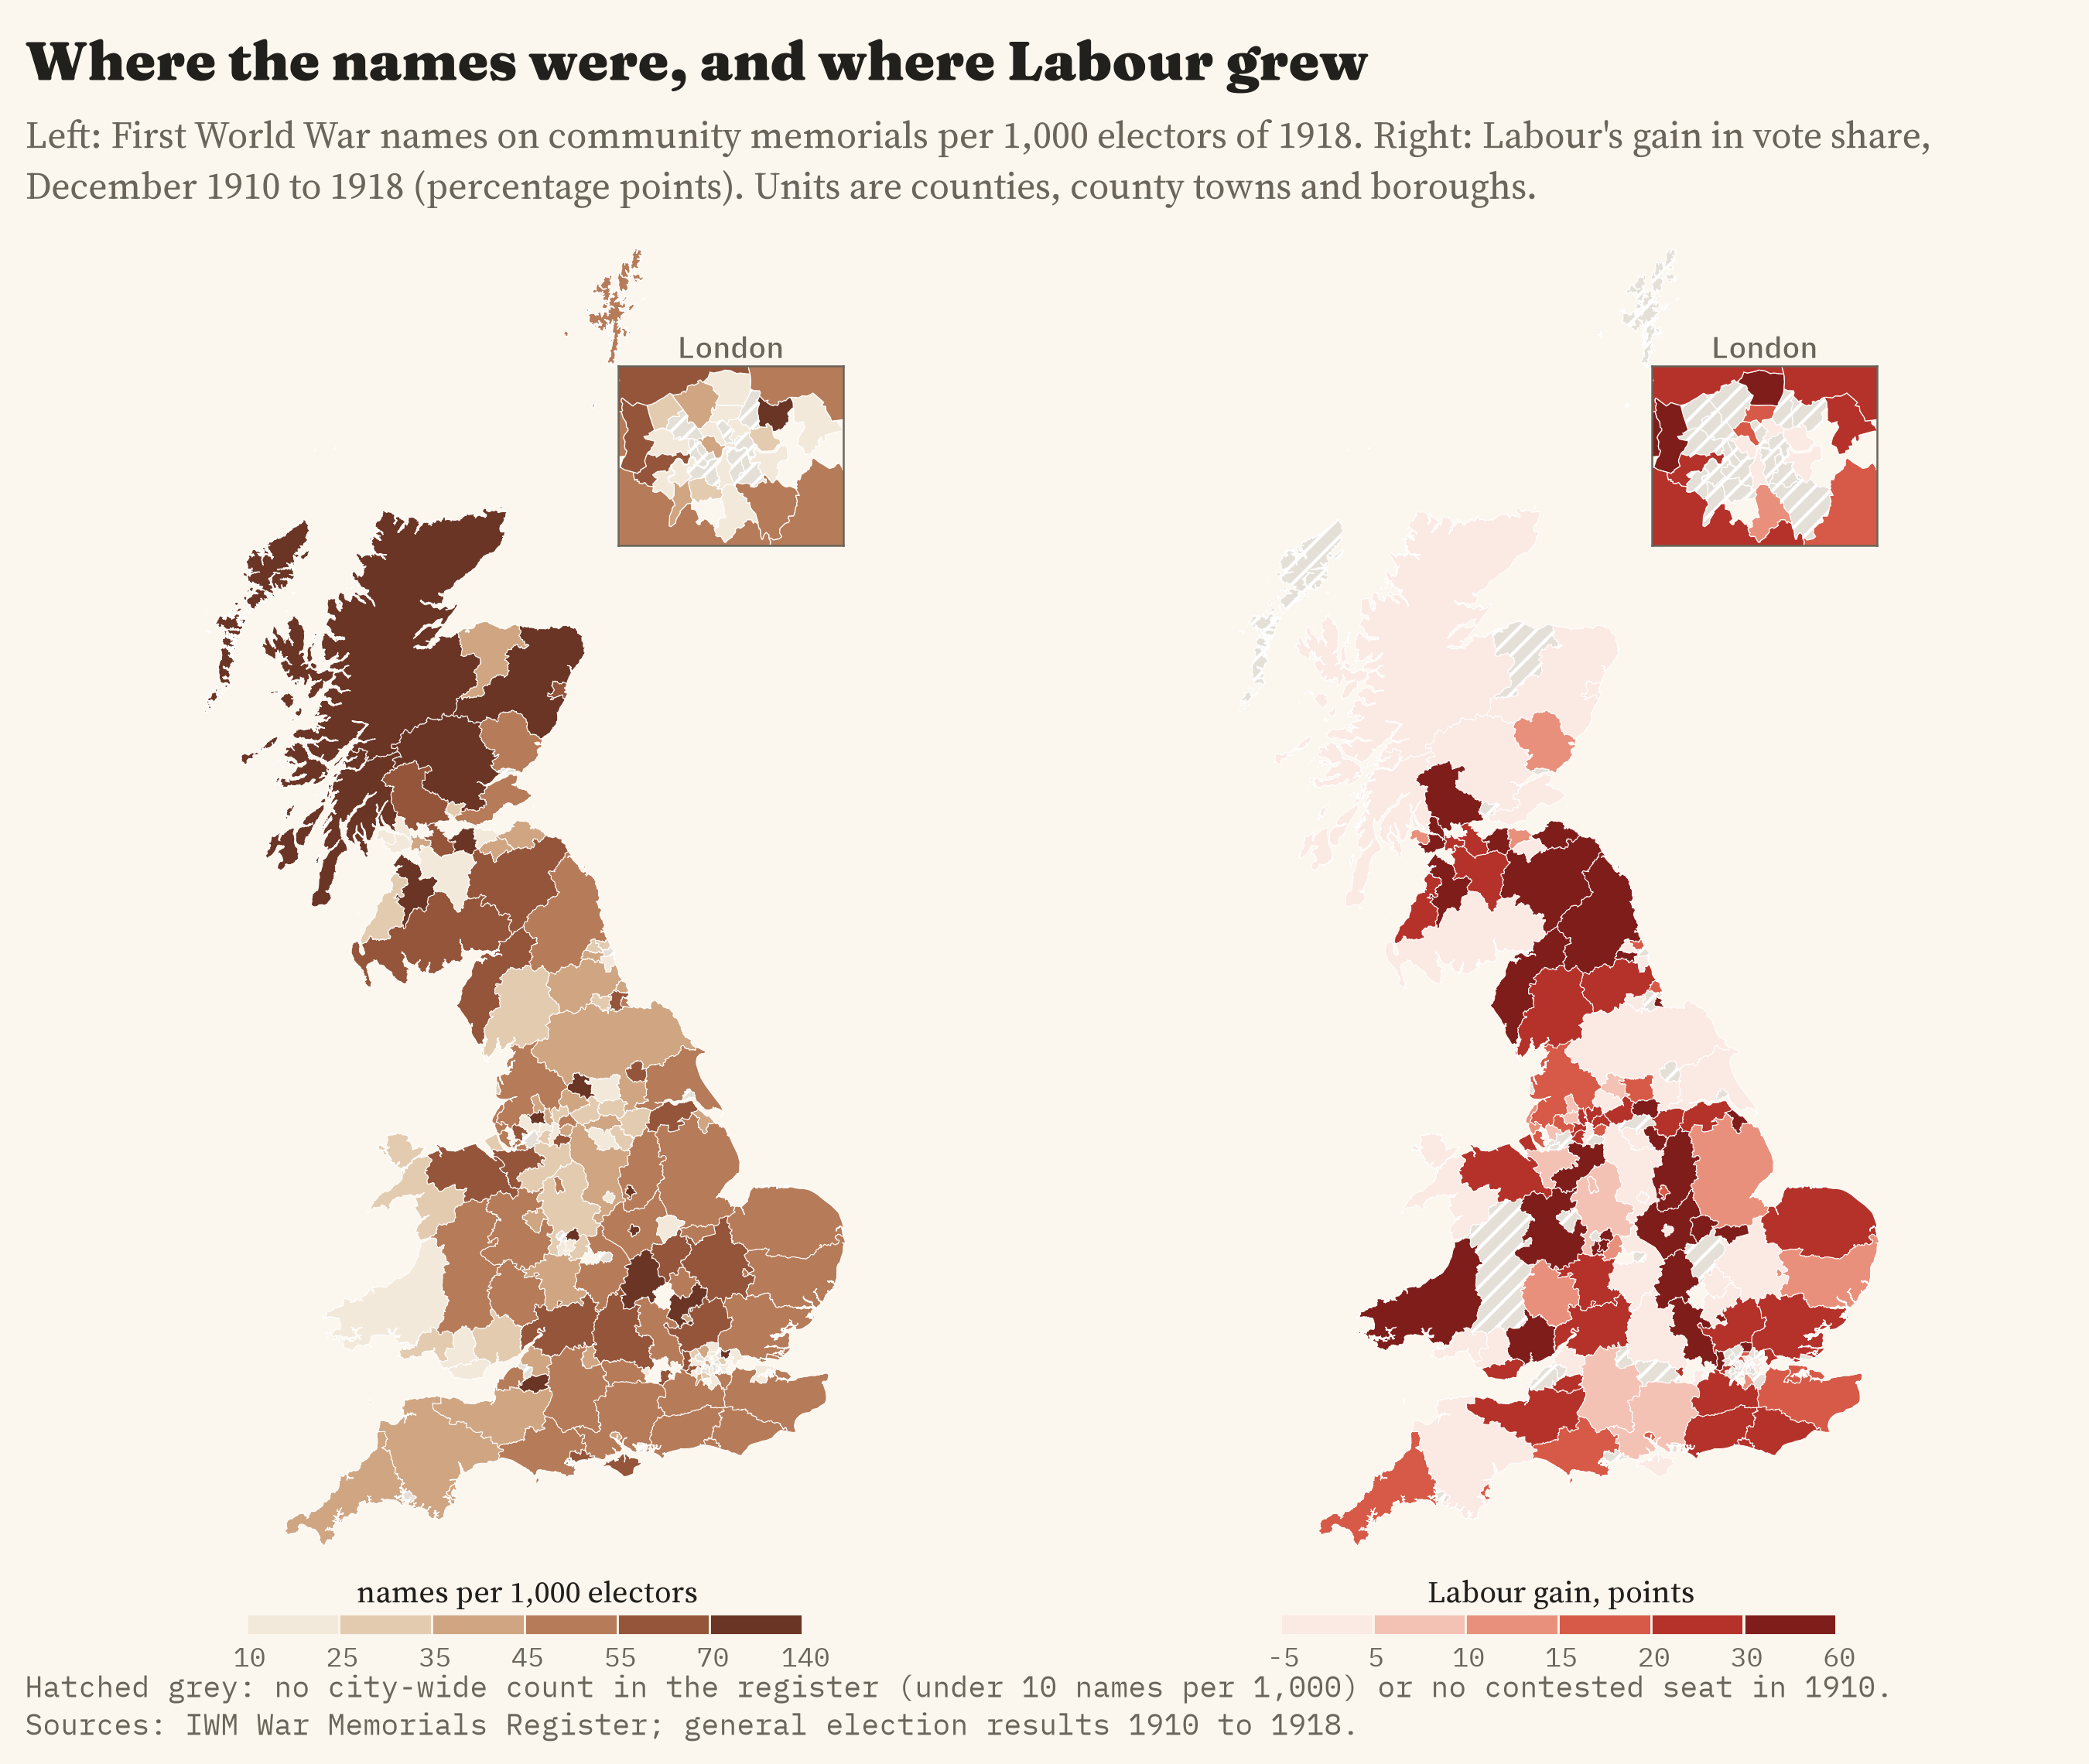
\includegraphics[width=0.95\textwidth]{f_maps.png}
\caption{Memorial names per 1,000 electors of 1918 (left) and the change in Labour's share of the vote from December 1910 to 1918 (right), by unit. Hatched: units below 10 names per 1,000 electors (no city-wide count) or without a contested seat in December 1910.}\label{fig:maps}\end{figure}

\subsection{The geography of the exposure}
The memorial rate is highest in the Highlands and islands of Scotland and in a band of rural English counties, and lowest in the Welsh valleys, parts of the industrial Midlands and many large towns (Figure~\ref{fig:maps}). Across the main sample it has a median of 44.2 names per 1,000 electors (interquartile range 27.7 to 54.7). It is negatively correlated with log electorate density ($r=$-$0.48$): rural units record more names per elector, partly because villages list their dead on a single cross while towns spread theirs over many memorials. It is positively but weakly correlated with the Second World War rate ($r=0.29$) and with the village rate, which uses present-day population as its denominator ($r=0.36$). The weak correlation with the village rate is a reminder that the two measures capture different things: the unit rate reflects how many of a unit's dead are recorded on community memorials at all, the village rate the intensity of loss among the places that do record them. The Western Isles has the highest rate of any unit (136 per 1,000 electors).

\subsection{The measurement problem in large towns}
The distribution of the exposure (Figure~\ref{fig:dist}) has a long lower tail of large towns and London boroughs with very few names per elector: Plymouth, Portsmouth, Southwark and Hammersmith and Fulham all have fewer than 3 names per 1,000 electors, against a median of 41 across all units. These are not places that escaped the war: their city-wide roll of honour is either not in the register or has no count, so that only a handful of small church and district memorials enter. A rate of 10 per 1,000, roughly a quarter of the national average, separates them cleanly from the rest. This was identified from the exposure alone, before any outcome model was run, and the 18 units below it are excluded from the main sample (Section~\ref{sec:design}) and restored as a robustness check.

\begin{figure}[tbp]\centering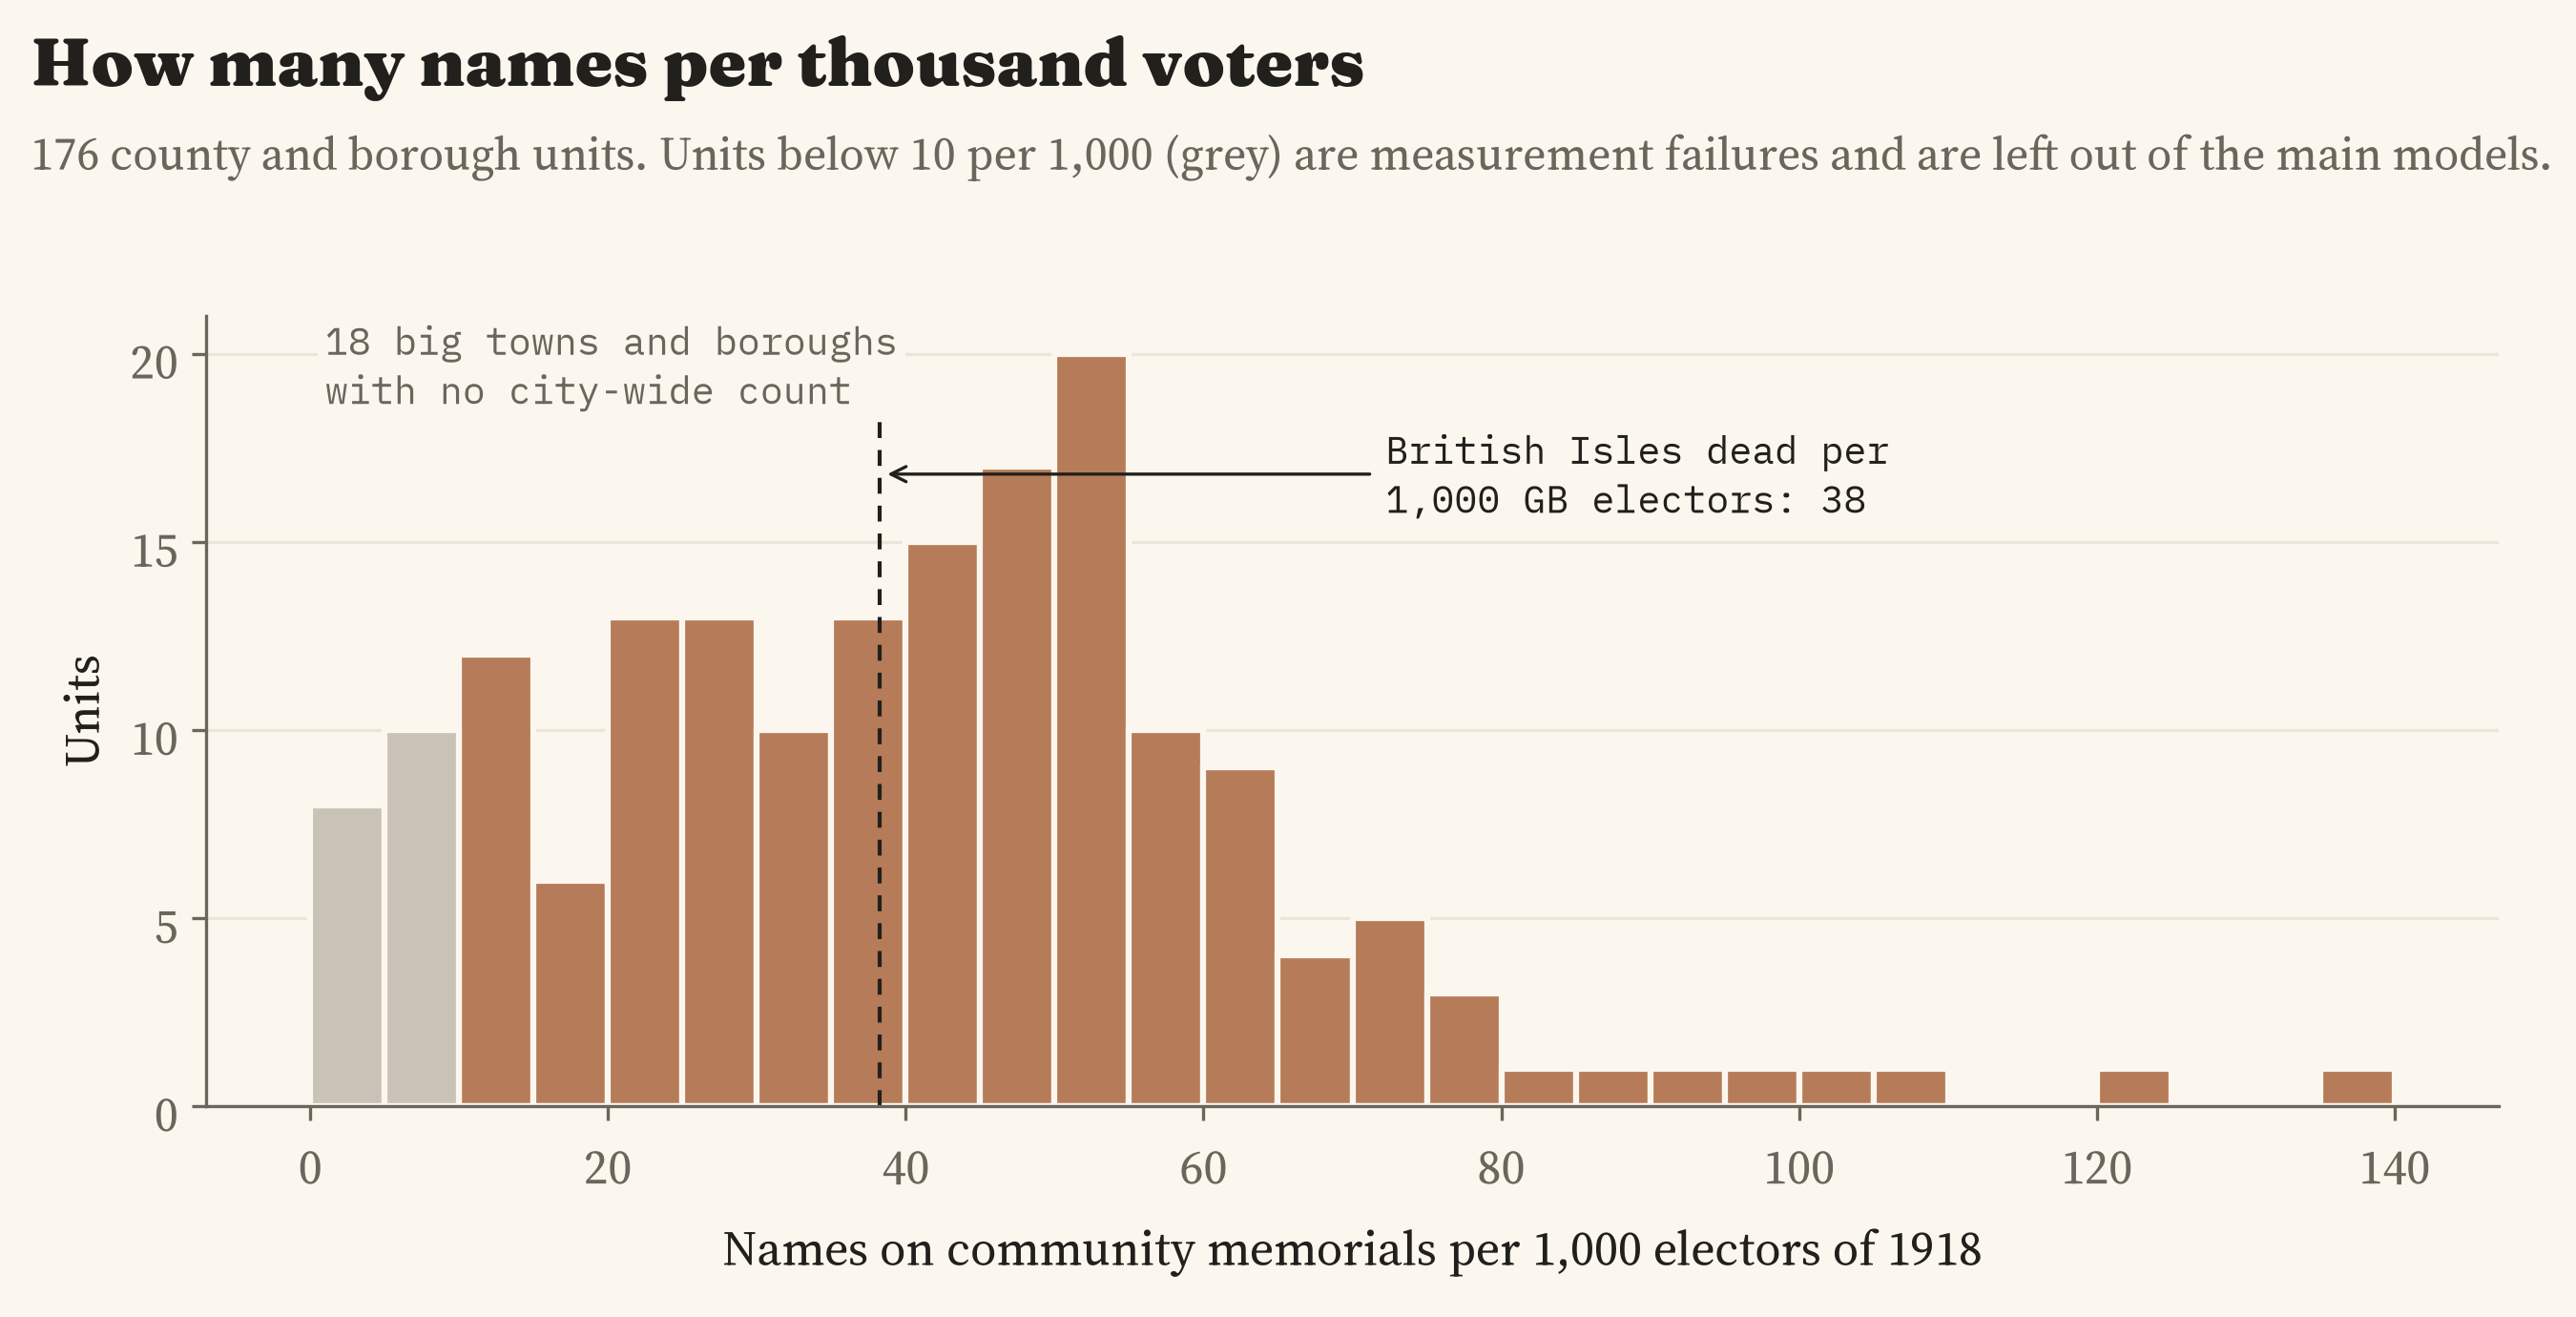
\includegraphics[width=0.9\textwidth]{f_dist.png}
\caption{Distribution of memorial names per 1,000 electors of 1918 across units. The dashed line is 744,000 British Isles dead per 1,000 Great Britain electors, a rough benchmark only.}\label{fig:dist}\end{figure}

\subsection{Validating the linkage}
Two checks address the linkage. First, as a test of the assignment of memorial places to constituencies used in the constituency-level robustness check, I take places whose name matches a 1918 borough seat and which lie within 15 km of that seat's point (so that namesakes elsewhere are excluded): of 365 such places, 337 (92.3\%) are assigned to the matching seat by the nearest-point rule and 354 (97.0\%) fall in the seat's unit. Most failures are suburbs of the same name as a neighbouring borough (Bromley-by-Bow in Tower Hamlets is not Bromley). Second, the county recorded for each memorial in the register agrees with the unit by a simple text match for 14,950 of 16,255 places (92.0\%); most disagreements are text differences such as Welsh names or ``County of Herefordshire''. The median distance from a memorial place to the nearest 1918 seat point is 9.9 km. The unit-level analysis requires only that places and seats fall in the right unit, which the checks suggest holds for the large majority; misassignment at the edges adds noise rather than bias in a known direction.

\section{Research design}\label{sec:design}
The analysis plan was written in the project notes before any outcome model was run or any outcome tabulated against the exposure. It is summarised here; two amendments, both made before any outcome model and both driven by the memorial data alone, are reported.

\textbf{Hypotheses.} H1 (radicalisation): higher losses, larger Labour gain from December 1910 to 1918. H2 (rally): higher losses, higher Coalition share in 1918. H3 (Liberal collapse): higher losses, larger Liberal fall. H4 (turnout): higher losses, different 1918 turnout. All tests are two-sided. Evidence against H1 was defined as a coefficient whose 95\% interval excludes a positive effect of one percentage point per standard deviation, or a placebo coefficient of similar size to the main one.

\textbf{Main specification.} For unit $u$ in region $r$,
\begin{equation}
Y_u = \alpha + \beta\, Z_u + \gamma \log D_u + \delta_1 \text{Lab}^{1910}_u + \delta_2 \text{Lib}^{1910}_u + \mu_r + \varepsilon_u,
\end{equation}
where $Z_u$ is the memorial rate standardised to mean zero and unit standard deviation, $D_u$ is electors per square kilometre, $\text{Lab}^{1910}$ and $\text{Lib}^{1910}$ are December 1910 shares, and $\mu_r$ are region fixed effects. Estimation is by ordinary least squares, unweighted, with HC3 heteroskedasticity-robust standard errors \citep{mackinnon1985}, which are preferable to clustering with only eleven regions \citep{cameron2015}. The estimating sample is units with at least 10 memorial names per 1,000 electors and contested seats in both elections. Across the four primary outcomes I report Holm-adjusted $p$ values \citep{holm1979}. Models are estimated with statsmodels \citep{seabold2010}.

\textbf{Amendments.} (1) The plan included the share of a unit's electorate in borough seats as a control; no source in the inputs identifies which 1918 seats were boroughs, and names do not (Penistone and Holderness were county divisions), so it was dropped and a quadratic in log density added as a check. (2) The exclusion of units below 10 names per 1,000 electors described above.

\textbf{Robustness.} Pre-specified variants: weighting by electorate; without the 1910 controls; with January 1910 as the baseline; a quadratic in density; without region effects; controlling for Second World War names per 1,000 electors (a proxy for local recording effort); five alternative exposures (log, rank, winsorised, the double-counted sum over all memorials, the median names per 1,000 present-day residents among villages of 100 to 5,000 people, names per seat); all units; units where at least half the memorial places have a count; units with at least two seats; without London, without Scotland, England only; dropping units with Cook's distance above $4/N$; leaving out each region in turn; and the constituency level, with memorial places assigned to the nearest 1918 seat within their unit, divided boroughs merged (464 seats or boroughs), unit-level 1910 controls and standard errors clustered by unit.

\textbf{Placebos.} If the memorial rate captures place characteristics that drove Labour's growth regardless of the war, it should also predict Labour's growth before the war. P1: the changes from 1906 to December 1910 and from January to December 1910 in Labour and Liberal shares, and the December 1910 levels, as outcomes. P2: Second World War memorial names per 1,000 electors, which cannot have affected the 1918 vote but share the recording process, as the exposure. P3: a permutation test, shuffling the exposure within regions 2,000 times.

\textbf{Threats to inference, stated in advance.} Four threats were identified when the plan was written. (i) Selection into service: death rates depended on who enlisted, and enlistment depended on occupation and on local social structure, which also shape partisanship. The pre-war placebo outcomes and the 1910 controls address the part of this that was already visible in pre-war voting; the part that was not cannot be addressed with these data. (ii) Rurality: villages record their dead more completely than towns and were less fertile ground for Labour; density is controlled, flexibly in a robustness check, and region effects compare like with like. (iii) Recording effort: a unit's memorial rate depends on how fully its memorials were catalogued with counts. The Second World War rate, which shares the recording process, enters as a control and as a placebo exposure, and the share of memorial places with a count defines a restricted sample. (iv) Mechanical composition: the dead are absent from the 1918 electorate, and their absence changes its composition; this is bounded in Section~\ref{sec:disc}.

\textbf{Interpretation.} The design compares places and is correlational. The coefficients describe how the vote changed in places that recorded more names, conditional on the controls; they are not estimates of the effect of a death on a family's vote, and the paper uses causal language only when discussing mechanisms that might produce the associations. Section~\ref{sec:disc} discusses what could produce the associations other than an effect of loss on votes.

\textbf{Power.} With 131 units and the residual variance of the main model, the standard error of the primary coefficient is 1.41 points per standard deviation. The design can therefore detect associations of about three points per standard deviation with conventional power, but not associations of one point, which would still be substantively interesting. A null on the secondary outcomes should be read with this in mind: the intervals for the Coalition share in particular are wide.

\section{Results}
\subsection{Primary outcomes}
Table~\ref{tab:main} reports the main specification. Labour's share in contested seats rose by an average of 17.6 points between December 1910 and 1918 across the 131 units in the sample (standard deviation 15.0). A one standard deviation higher memorial rate, 21.6 names per 1,000 electors, is associated with a Labour gain 2.90 points smaller (95\% CI 0.13 to 5.68; $p=0.040$), or $-$1.35 points per 10 names per 1,000 electors: about a fifth of a standard deviation of the outcome. The within-region permutation test gives $p=0.027$. After Holm adjustment across the four primary outcomes, $p=0.16$. The coefficient is negative, the opposite of H1, and its interval excludes the pre-specified positive effect of one point.

\begin{table}[tbp]\centering\small\caption{Main specification: memorial names per 1,000 electors (standardised) and the four primary outcomes. OLS on county and borough units with region fixed effects, log density and December 1910 Labour and Liberal shares; HC3 standard errors in parentheses.}\label{tab:main}\begin{tabular}{lrrrr}\toprule & Labour change & Coalition share & Liberal change & Turnout\\\midrule
Memorial rate (per SD) & $-$2.90 & 3.67 & $-$1.06 & $-$0.45\\
 & (1.41) & (2.81) & (2.05) & (0.84)\\
95\% CI & [$-$5.7, $-$0.1] & [$-$1.8, 9.2] & [$-$5.1, 3.0] & [$-$2.1, 1.2]\\
$p$ & 0.040 & 0.191 & 0.605 & 0.591\\
Holm-adjusted $p$ & 0.160 & 0.573 & 1.000 & 1.000\\
Per 10 names per 1,000 & $-$1.35 & 1.70 & $-$0.49 & $-$0.21\\
Mean of outcome & 17.6 & 51.8 & $-$16.7 & 57.4\\
$N$ (units) & 131 & 131 & 131 & 131\\
$R^2$ & 0.33 & 0.24 & 0.26 & 0.36\\
\bottomrule\end{tabular}\end{table}

To put the magnitude in context: moving from a unit at the first quartile of the memorial rate (28 per 1,000) to one at the third (55) corresponds to about 1.3 standard deviations, or a Labour gain roughly 3.6 points smaller, against an average gain of 17.6 points. Without controls the association is weaker ($-$1.31, $p=0.38$), because high-rate units are rural and Labour gained less in rural areas regardless: the controls for density and region do not create the association but sharpen it, by comparing units of similar character within the same region.

The other primary outcomes are imprecise. The Coalition share is higher by 3.7 points per standard deviation (CI $-$1.8 to 9.2), the Liberal change is $-$1.1 ($-$5.1 to 3.0) and 1918 turnout $-$0.5 ($-$2.1 to 1.2). None of H2 to H4 finds support, and none can be ruled out at the size of a few points. Figure~\ref{fig:scatter} shows the primary association after partialling out the controls: it is not driven by a handful of units, although the units with the highest adjusted rates (Nottingham, Walsall and Leicester, whose count is a city-and-county book of remembrance) are visible at the right.

\begin{figure}[tbp]\centering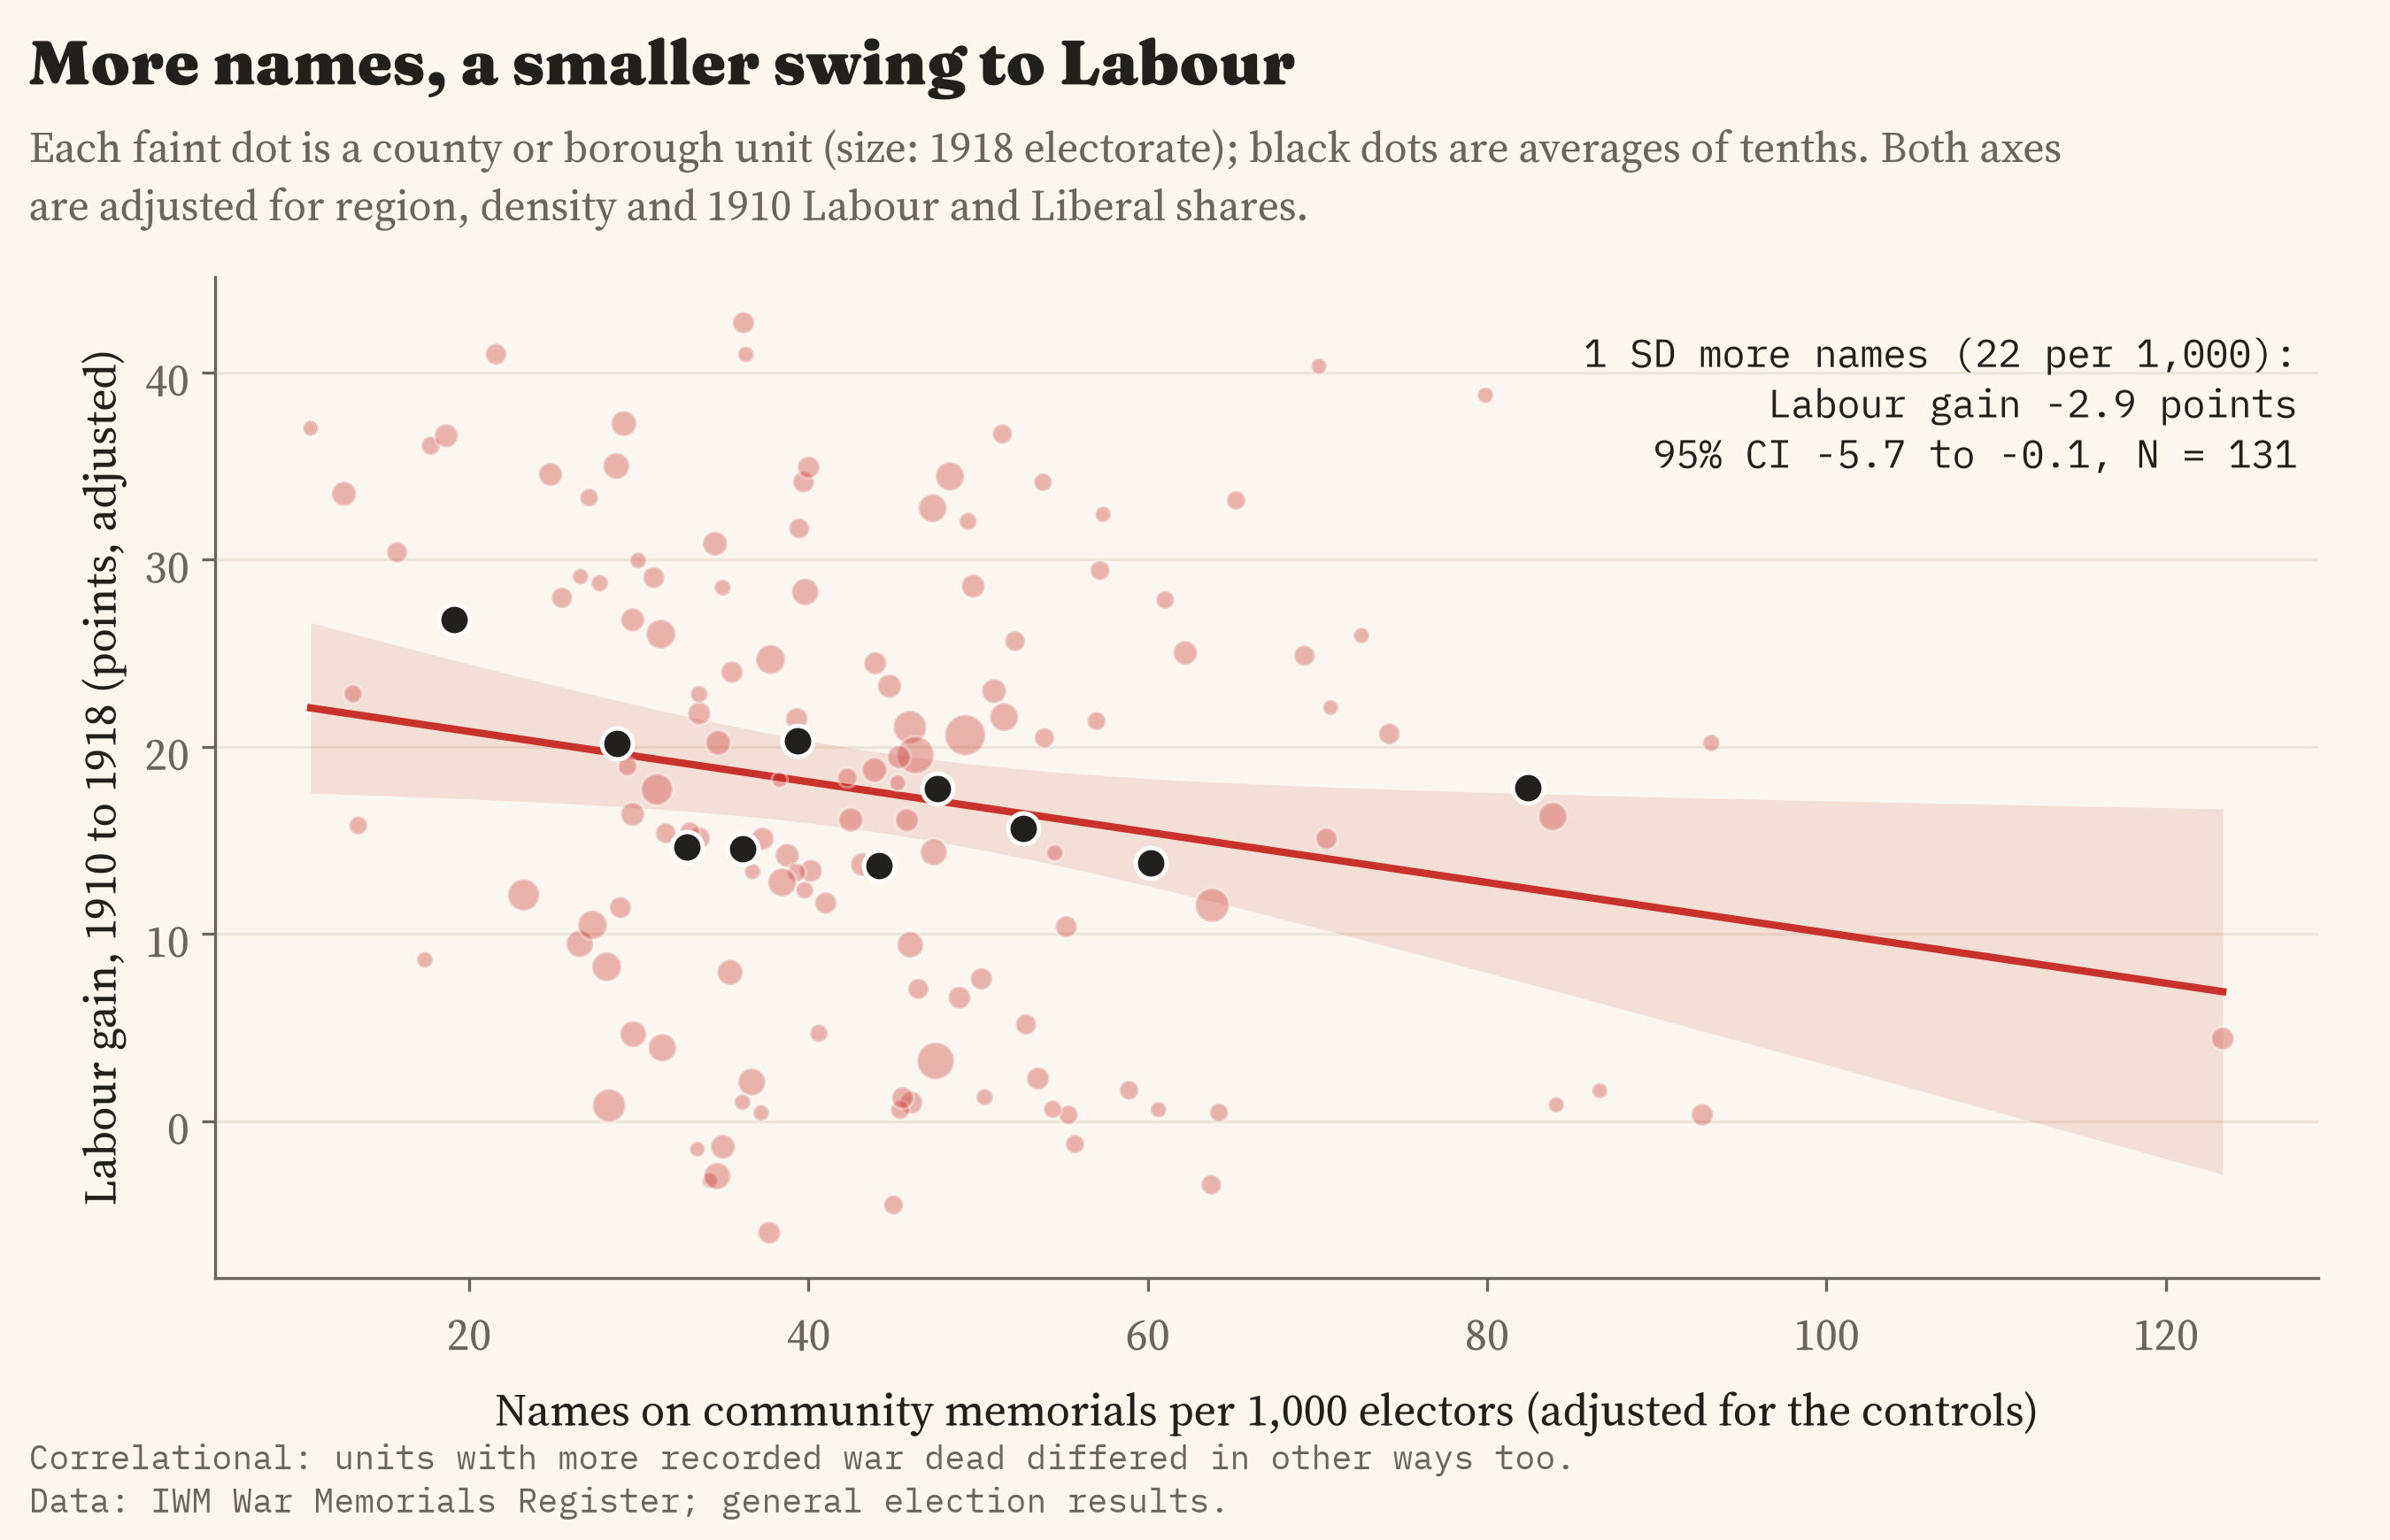
\includegraphics[width=0.95\textwidth]{f_scatter.png}
\caption{Labour's gain from December 1910 to 1918 against memorial names per 1,000 electors, both residualised on the controls and region effects (Frisch to Waugh). Dot size: 1918 electorate. Black: means of deciles. Line: OLS fit with 95\% interval.}\label{fig:scatter}\end{figure}

\subsection{Pre-war placebos and the post-war path}
If the exposure merely picked out places where Labour was growing anyway, it should predict the pre-war trend. It does not (Table~\ref{tab:placebo}, Figure~\ref{fig:path}). The coefficients for the change in Labour's share from 1906 to December 1910 ($-$0.67, CI $-$2.58 to 1.23) and between the two 1910 elections (0.32), and for the level of the Labour and Liberal vote in December 1910, are all small and far from significance. The pre-war window is short and Labour stood in few seats before 1914, so these tests have limited power to detect slow-moving differences, but they rule out pre-existing trends of the size of the post-war gap. The Second World War memorial rate, which shares the recording process but not the timing, does not predict the 1918 Labour change ($-$0.79, CI $-$8.30 to 6.71).

\begin{table}[tbp]\centering\footnotesize\caption{Placebo and falsification tests. Rows 1 to 6: pre-war outcomes regressed on the First World War memorial rate (controls: density, region and the shares at the start of each window; for 1910 levels, density and region). Rows 7 to 10: the Second World War memorial rate as the exposure for the primary outcomes.}\label{tab:placebo}\begin{tabular}{p{8.3cm}rrrr}\toprule Test & Coef. & 95\% CI & $p$ & $N$\\\midrule
Labour change 1906 to Dec 1910 & $-$0.67 & [$-$2.58, 1.23] & 0.488 & 134\\
Liberal change 1906 to Dec 1910 & 0.51 & [$-$1.28, 2.29] & 0.576 & 134\\
Labour change Jan to Dec 1910 & 0.32 & [$-$0.86, 1.49] & 0.598 & 136\\
Liberal change Jan to Dec 1910 & $-$0.13 & [$-$1.11, 0.85] & 0.791 & 136\\
Labour share Dec 1910 (level) & 0.18 & [$-$2.84, 3.20] & 0.909 & 136\\
Liberal share Dec 1910 (level) & 0.33 & [$-$1.61, 2.27] & 0.740 & 136\\
Second World War names per 1,000 as the exposure: Labour share change, Dec 1910 to 1918 & $-$0.79 & [$-$8.30, 6.71] & 0.836 & 131\\
Second World War names per 1,000 as the exposure: Coalition (coupon) share 1918 & 2.63 & [$-$0.37, 5.62] & 0.085 & 131\\
Second World War names per 1,000 as the exposure: Liberal share change, Dec 1910 to 1918 & $-$0.20 & [$-$7.92, 7.52] & 0.960 & 131\\
Second World War names per 1,000 as the exposure: Turnout 1918 & $-$0.70 & [$-$2.06, 0.67] & 0.319 & 131\\
Permutation within region, Labour change 1910 to 1918 (2,000 draws) & $-$2.90 & & 0.027 & 131\\
\bottomrule\end{tabular}\end{table}

After 1918 the gap widens. Relative to December 1910, Labour's gain by 1922 is 4.76 points smaller per standard deviation (CI 2.10 to 7.43; $p<0.001$), by 1923 $-$4.58 and by 1924 $-$2.69 (Table~\ref{tab:later}). The Liberal share mirrors this: in 1918 the Liberal change is not associated with the exposure, but by 1922 the Liberals did 4.44 points better per standard deviation (CI 0.80 to 8.07), declining to 2.59 in 1924. These are pre-specified secondary outcomes, reported without adjustment; they are correlated with each other because they share the 1910 baseline.

\begin{table}[tbp]\centering\small\caption{Secondary outcomes: change in Labour and Liberal shares from December 1910 to each later election, and the all-Conservative change to 1918 (main specification; unadjusted $p$).}\label{tab:later}\begin{tabular}{lrrrr}\toprule Outcome & Coef. & 95\% CI & $p$ & $N$\\\midrule
Labour change to 1922 & $-$4.76 & [$-$7.43, $-$2.10] & <0.001 & 136\\
Labour change to 1923 & $-$4.58 & [$-$7.23, $-$1.92] & <0.001 & 134\\
Labour change to 1924 & $-$2.69 & [$-$4.57, $-$0.81] & 0.005 & 136\\
Liberal change to 1922 & 4.44 & [0.80, 8.07] & 0.017 & 136\\
Liberal change to 1923 & 3.63 & [0.85, 6.41] & 0.011 & 134\\
Liberal change to 1924 & 2.59 & [0.04, 5.14] & 0.047 & 136\\
Conservative (all) change to 1918 & 1.73 & [$-$3.86, 7.32] & 0.545 & 131\\
\bottomrule\end{tabular}\end{table}

\begin{figure}[tbp]\centering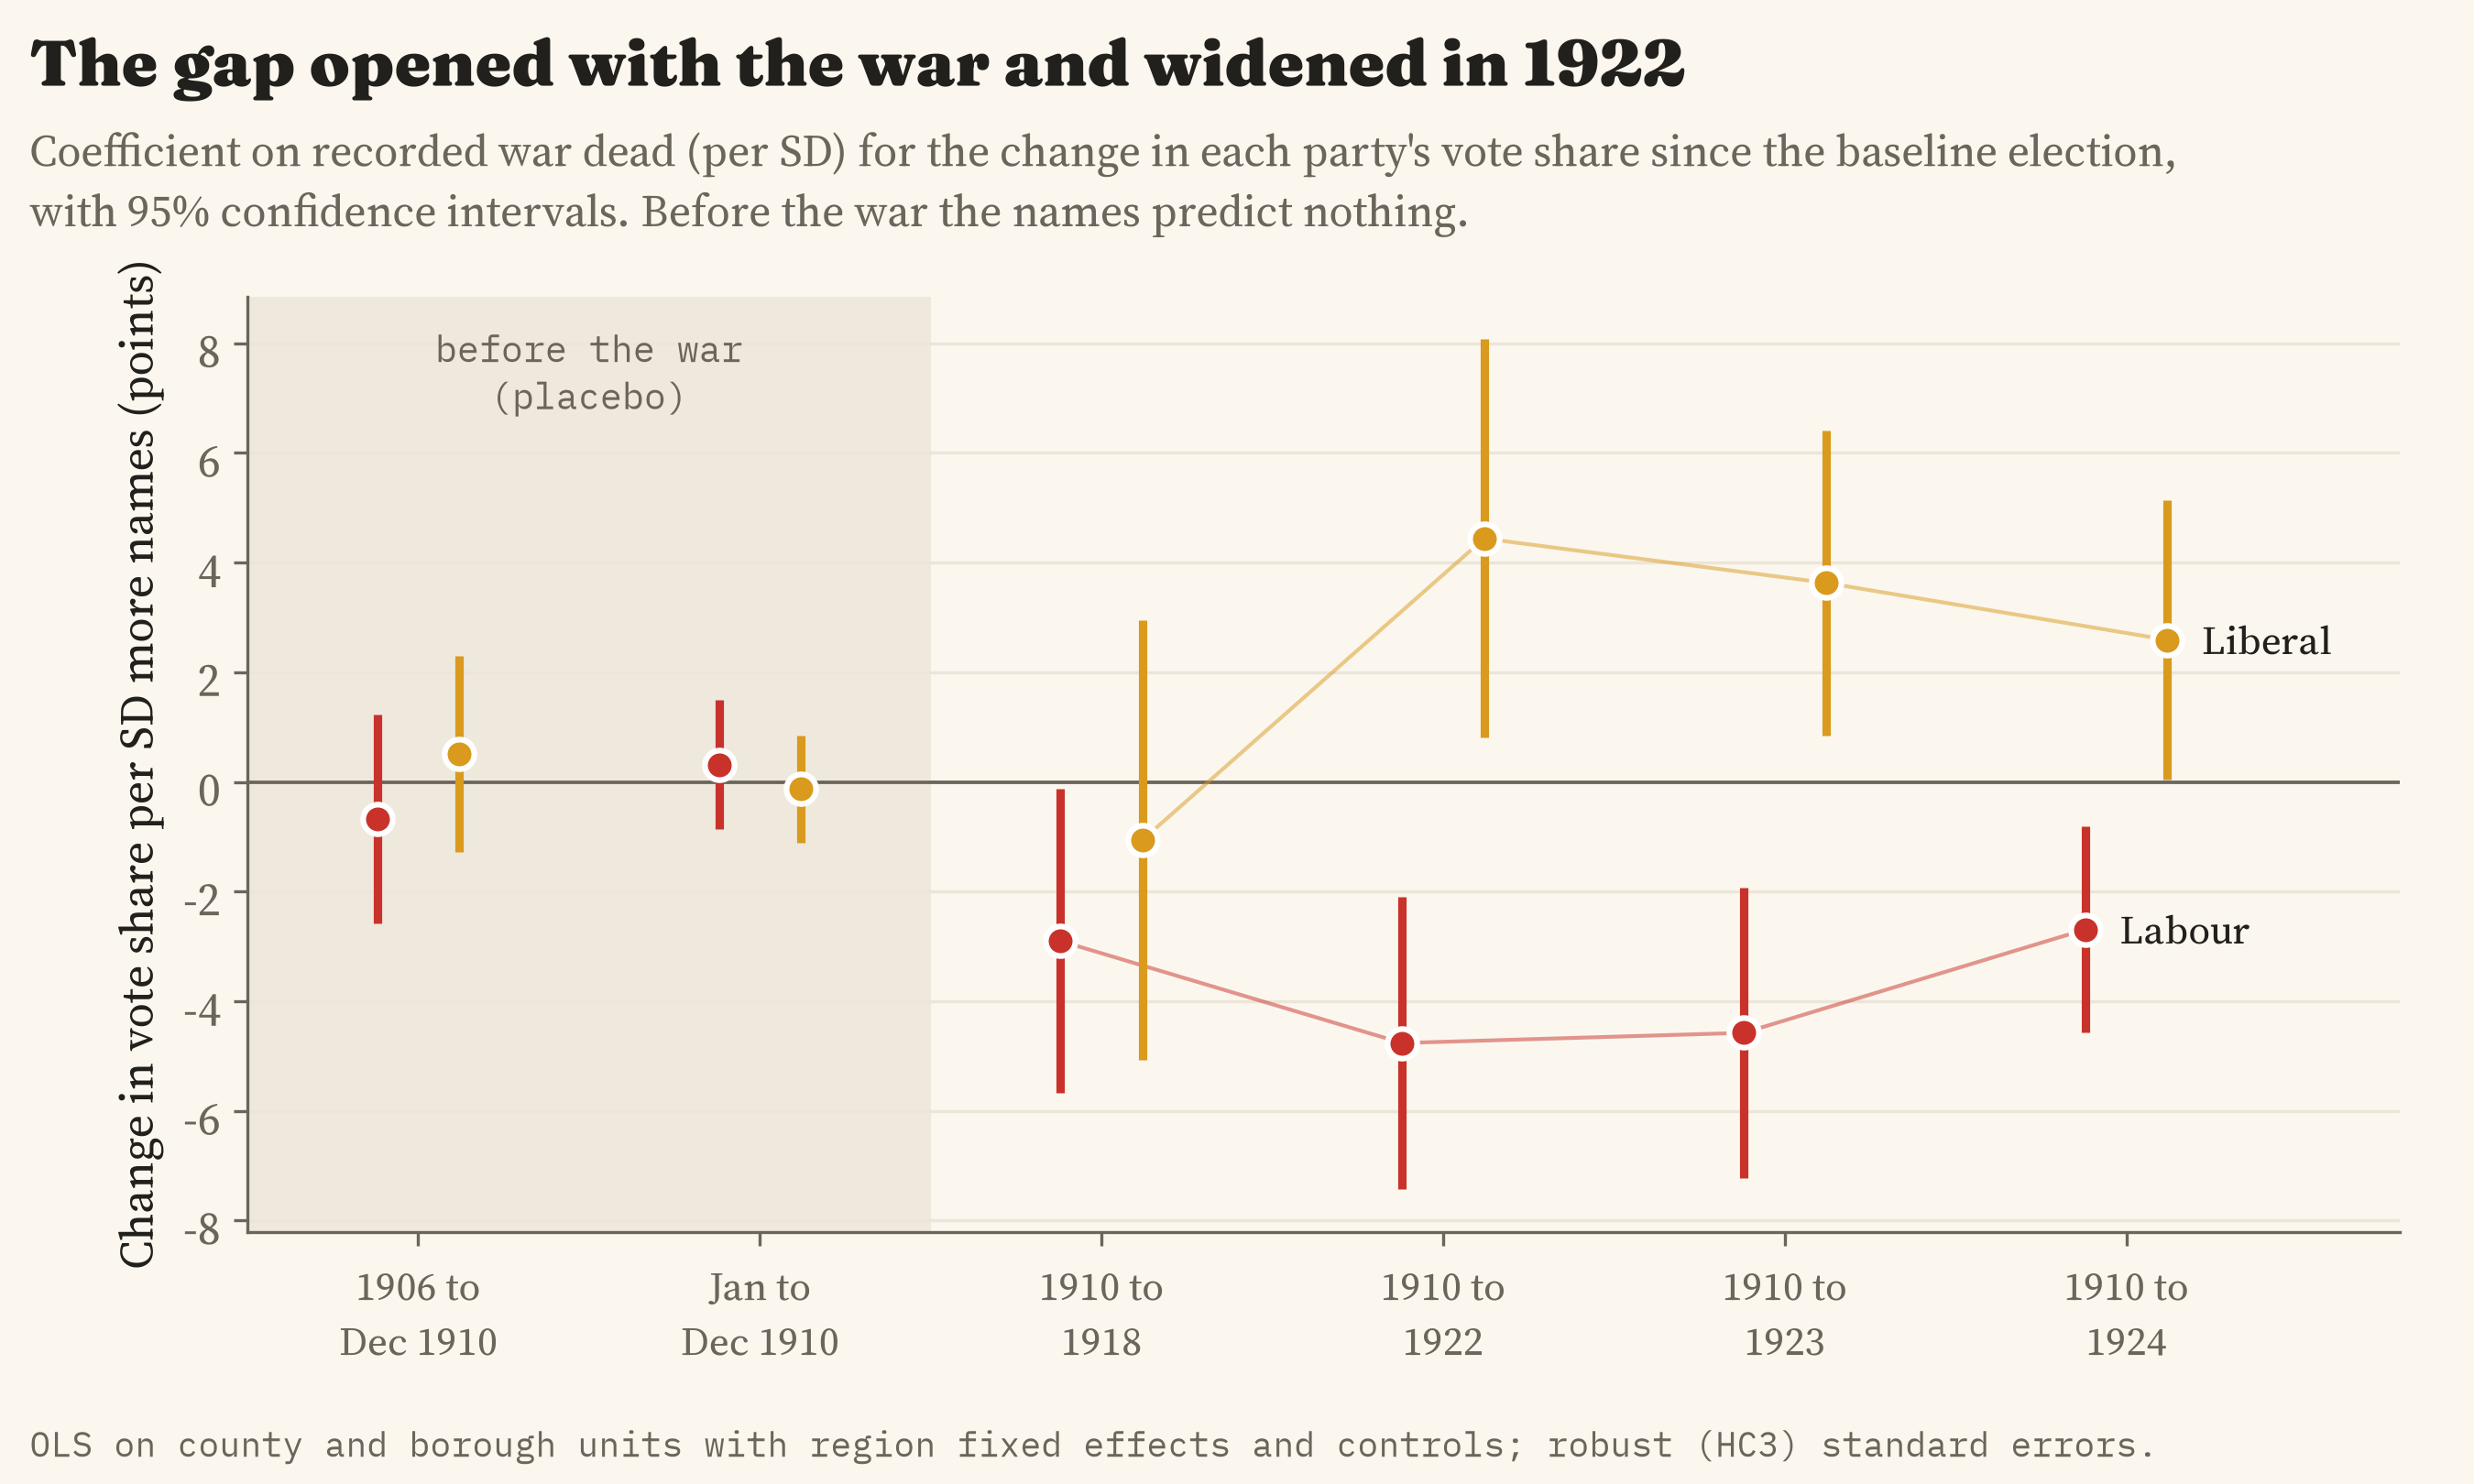
\includegraphics[width=0.95\textwidth]{f_path.png}
\caption{Coefficients (per standard deviation of the memorial rate) for the change in Labour and Liberal shares from each baseline, with 95\% intervals. The shaded pre-war changes are placebos (controls: density, region and the shares at the start of each window).}\label{fig:path}\end{figure}

\section{Robustness}
Figure~\ref{fig:robust} and Table~\ref{tab:robust} report the pre-specified variants for all four primary outcomes. For the Labour change, all 21 variants give negative coefficients, between $-$3.95 and $-$1.94; 8 have 95\% intervals excluding zero. Two qualifications apply to that count: the restriction to units where at least half the memorial places have a count removes no unit from the estimating sample, so it repeats the main estimate, and the seat-level model restricted to seats with 10 or more names per 1,000 electors was added alongside the planned seat-level model rather than specified in advance. Most variants, in other words, cannot distinguish the association from zero. The estimate is largest when influential units are dropped and when the sample is restricted to units with at least two seats, and smallest with a quadratic in density ($-$1.94, $p=0.14$), without region effects, and with the log or rank of the exposure ($p$ of about 0.11). The double-counted sum over all memorials gives a stronger association; the village rate, available for only 81 units, gives a similar point estimate with a wide interval. The constituency-level models, with 338 seats or merged boroughs, give $-$2.51 (CI $-$4.24 to $-$0.78). Leaving out each region in turn gives coefficients from $-$3.37 to $-$2.17, 6 of 11 significant at 5\%; the estimate is weakest without the East Midlands ($-$2.17, $p=0.20$), which contains two of the highest-rate units, and without Scotland ($-$2.40), where memorial rates were high.

Restoring the 18 low-count units gives $-$2.63 ($p=0.06$), weighting by electorate $-$2.61 ($p=0.06$), and controlling for the Second World War rate $-$2.86 ($p=0.06$). The Coalition coefficient is positive in every variant and significant at the constituency level (3.88, CI 1.46 to 6.30) and after dropping influential units, but not in the main specification. The Liberal and turnout coefficients are small and unstable in sign.

\begin{figure}[tbp]\centering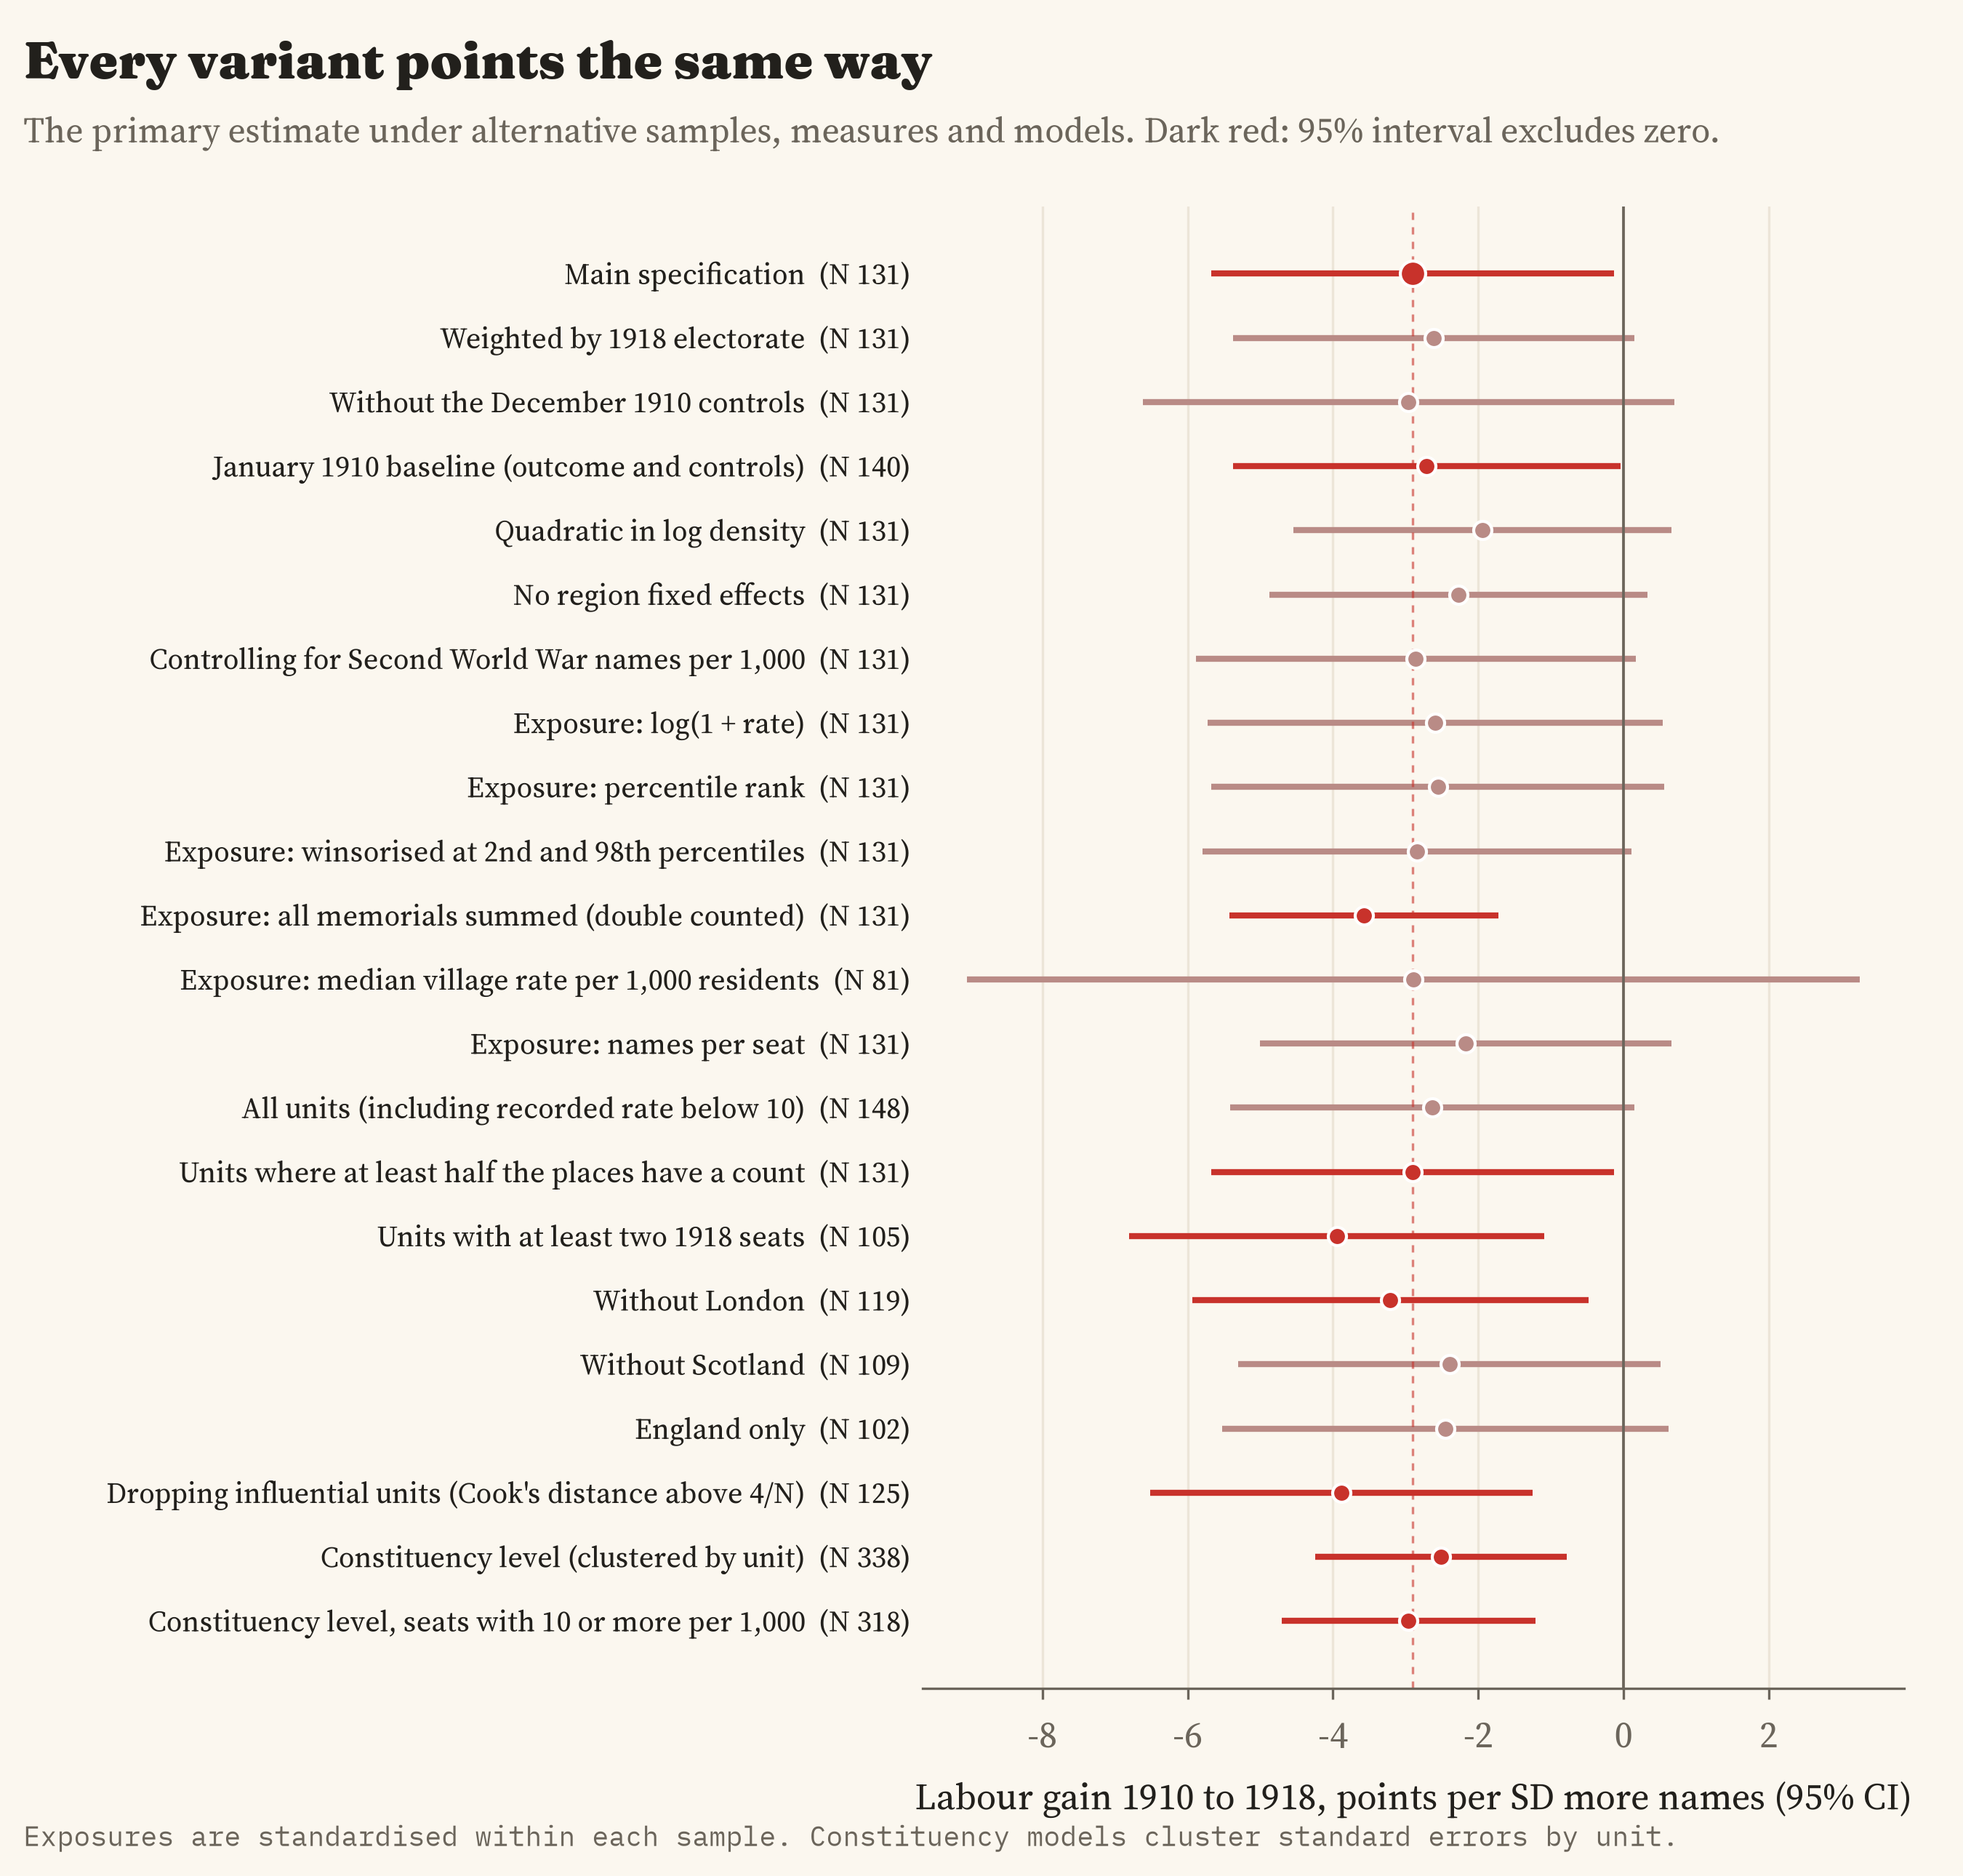
\includegraphics[width=0.9\textwidth]{f_robust.png}
\caption{The primary coefficient under the pre-specified variants, with 95\% intervals. Exposures are standardised within each sample.}\label{fig:robust}\end{figure}

\begin{table}[tbp]\centering\scriptsize\caption{Robustness: coefficient per SD of the exposure ($p$ in parentheses) under each variant (all pre-specified except the seat-level model restricted to 10 or more names per 1,000). $N$ is for the Labour change.}\label{tab:robust}\begin{tabular}{p{6.2cm}rrrrr}\toprule Variant & Labour & Coalition & Liberal & Turnout & $N$\\\midrule
Main specification & $-$2.90 (0.040) & 3.67 (0.191) & $-$1.06 (0.605) & $-$0.45 (0.591) & 131\\
Weighted by 1918 electorate & $-$2.61 (0.064) & 3.64 (0.153) & $-$2.51 (0.180) & $-$0.26 (0.779) & 131\\
Without the December 1910 controls & $-$2.96 (0.113) & 2.41 (0.314) & $-$0.99 (0.642) & $-$0.54 (0.528) & 131\\
January 1910 baseline (outcome and controls) & $-$2.71 (0.046) & 3.52 (0.166) & $-$0.87 (0.658) & $-$0.34 (0.677) & 140\\
Quadratic in log density & $-$1.94 (0.143) & 3.34 (0.241) & $-$2.16 (0.235) & $-$0.04 (0.956) & 131\\
No region fixed effects & $-$2.27 (0.087) & 2.65 (0.329) & $-$2.14 (0.234) & $-$0.70 (0.340) & 131\\
Controlling for Second World War names per 1,000 & $-$2.86 (0.064) & 3.18 (0.266) & $-$1.07 (0.606) & $-$0.29 (0.751) & 131\\
Exposure: log(1 + rate) & $-$2.59 (0.105) & 4.06 (0.125) & $-$1.64 (0.388) & $-$0.59 (0.492) & 131\\
Exposure: percentile rank & $-$2.56 (0.108) & 3.36 (0.220) & $-$1.69 (0.397) & $-$0.46 (0.583) & 131\\
Exposure: winsorised at 2nd and 98th percentiles & $-$2.84 (0.059) & 3.79 (0.202) & $-$1.25 (0.549) & $-$0.34 (0.682) & 131\\
Exposure: all memorials summed (double counted) & $-$3.57 (<0.001) & 0.81 (0.578) & 1.01 (0.271) & $-$0.74 (0.159) & 131\\
Exposure: median village rate per 1,000 residents & $-$2.89 (0.356) & 1.77 (0.625) & 0.06 (0.986) & $-$1.50 (0.053) & 81\\
Exposure: names per seat & $-$2.17 (0.133) & 3.35 (0.316) & $-$1.22 (0.514) & 0.06 (0.936) & 131\\
All units (including recorded rate below 10) & $-$2.63 (0.063) & 3.40 (0.235) & $-$1.90 (0.335) & $-$0.20 (0.812) & 148\\
Units where at least half the places have a count & $-$2.90 (0.040) & 3.67 (0.191) & $-$1.06 (0.605) & $-$0.45 (0.591) & 131\\
Units with at least two 1918 seats & $-$3.95 (0.007) & 4.62 (0.130) & $-$0.54 (0.787) & $-$1.07 (0.251) & 105\\
Without London & $-$3.21 (0.021) & 3.74 (0.195) & $-$0.67 (0.754) & $-$0.47 (0.587) & 119\\
Without Scotland & $-$2.40 (0.106) & 2.45 (0.442) & $-$1.87 (0.262) & 0.28 (0.732) & 109\\
England only & $-$2.45 (0.118) & 2.36 (0.496) & $-$2.59 (0.122) & 0.35 (0.686) & 102\\
Dropping influential units (Cook's distance above 4/N) & $-$3.89 (0.004) & 3.59 (0.022) & $-$0.83 (0.590) & 0.25 (0.735) & 125\\
Constituency level (clustered by unit) & $-$2.51 (0.005) & 3.88 (0.002) & 0.22 (0.865) & 0.12 (0.779) & 338\\
Constituency level, seats with 10 or more per 1,000 & $-$2.96 (<0.001) & 2.94 (0.014) & 0.66 (0.606) & $-$0.08 (0.875) & 318\\
\bottomrule\end{tabular}\end{table}

\subsection{Checks added after review}\label{sec:review}
The following checks were added after the main results were known, in response to referee-style questions, and are exploratory. The 10 per 1,000 threshold for excluding low-count units matters for precision but not for the estimate: thresholds of 5, 15 and 20 give $-$2.99 ($p=0.04$), $-$2.80 ($p=0.05$) and $-$2.21 ($p=0.12$), and no threshold gives $-$2.63 ($p=0.06$). The amendment that set the threshold is recorded in the project notes as made before any outcome model was run; the notes are the only record of that order. Controlling for the share of memorial places with a count, a direct measure of recording completeness, gives $-$2.28 ($p=0.10$). The denominator checks are reported in Section~\ref{sec:disc}. Taken together, these checks leave the sign and rough size of the association unchanged and confirm that its statistical significance is marginal.

\subsection{Exploratory: candidacy and heterogeneity}
The following analyses were not in the plan. Labour's change in vote share combines whether Labour stood and how well it did. A higher memorial rate is associated with a $-$5.5 point lower share of a unit's 1918 seats with a Labour candidate (CI $-$13.2 to 2.1). Restricted to the 112 units where Labour stood at least once in 1918, the coefficient on the Labour change falls to $-$0.99 (CI $-$3.53 to 1.54). Much of the association therefore appears to run through where Labour contested, which is a decision of local parties and trade unions as much as of voters. In England alone the coefficient is $-$2.45 ($N=102$), and it is $-$2.77 in the more densely populated half of units and $-$1.53 in the less dense half, both with wide intervals.

\subsection{The Coalition and turnout}
The Coalition share is the outcome most directly tied to the rally hypothesis, and its coefficient is positive in the main specification and in every variant, from 0.81 to 4.62 points per standard deviation. It is significant at the constituency level and after dropping influential units, but not in the main specification, where the interval is wide because the Coalition share varies greatly with whether a couponed Liberal or Conservative stood and whether the seat was a straight fight. The Second World War placebo exposure also has a positive, marginal coefficient for the Coalition share (2.63, $p=0.09$), which suggests that part of the Coalition association reflects the kind of place that records its dead fully, rather than the dead of 1914 to 1918. The evidence for H2 is therefore suggestive at most. Turnout in 1918 is unrelated to the memorial rate in the main specification and in all but one variant (the village rate, $p=0.05$).

\section{Discussion}\label{sec:disc}
\subsection{What the association does and does not show}
The central finding is negative for the radicalisation account: in Britain, places that recorded more war dead per elector did not move more to Labour in 1918, and by 1922 they had moved noticeably less. The finding is consistent with the rally mechanism, in the weak form that heavy local loss went with loyalty to the parties that had led the war, and with \citet{lawrence2003}'s picture of a post-war political culture that recoiled from violence and radicalism. It is not consistent with the Italian and German pattern \citep{acemoglu2022,dejuan2024}, perhaps because Britain was a victor, because its post-war crisis was milder, or because Labour, unlike the Italian Socialists, did not oppose the war.

But the design cannot separate loss from the circumstances that produced it, and the most important of these points in the same direction as the finding. Death rates depended on enlistment, and enlistment depended on occupation: miners, munitions workers, shipbuilders, railwaymen and agricultural labourers were often retained at home, while clerks, shop workers and the professional classes volunteered and died at higher rates \citep{winter1977,dewey1984}. The industrial places with retained workforces, notably the coalfields, were also where Labour grew fastest after 1918. A negative association between recorded deaths and Labour growth is what this composition alone would produce, without any effect of loss on votes. I have no measure of industrial structure for 1918; region effects, density and the pre-war vote absorb some of it, and the null pre-war placebos show that the exposure did not pick up places where Labour was already growing between 1906 and 1910, but places can differ in their potential for post-war growth without having shown it before. The finding is best read as: the places that gave most men to the war were not the places where Labour advanced, for reasons that may be compositional rather than attitudinal.

A mechanical channel also exists. The dead did not vote. If they would otherwise have voted Labour at a higher rate than the rest of the electorate, their absence alone lowers Labour's share. The memorial rate is 22 names per 1,000 electors per standard deviation, about 2.2\% of the electorate; even if every dead man would have voted Labour and no one else had, removing them could lower Labour's share by at most about that amount, and realistically by a fraction of it. This bound assumes the dead would have turned out like other electors. Composition of this kind could therefore account for much of the 1918 coefficient in the extreme case, and realistically for a small part of it, but it cannot account for the 1922 and 1923 coefficients, which exceed the bound.

\subsection{Relation to other evidence}
The null result for turnout differs from the finding of \citet{carozzi2023} that English parishes with more war deaths had higher turnout between the wars. The designs differ in several ways: they use individual death records geocoded to parishes and instrument deaths with the battalion-level fortunes of local units, while this paper uses memorial counts aggregated to large units and a single post-war election, in which turnout was shaped by the service vote and the hurried register. The 1918 turnout outcome is a poor test of a civic-capital mechanism that, on their account, built up through the 1920s. The results are compatible: loss could raise participation without favouring Labour.

For the historiography, the findings sit more easily with accounts that stress continuity and local political organisation than with those that see the war as a radicalising experience that swept voters to Labour. On most accounts Labour's advance in 1918 was strongest where it had organisation and union strength \citep{mckibbin1974,tanner1990}, and these were not, on average, the places that gave most men to the war. That the gap widened in 1922, after the Coalition had broken up and the Liberals partially reunited, suggests that the high-loss places returned to the Liberals, or stayed with them, rather than moving to Labour once the coupon no longer structured the choice. The decomposition by candidacy points to the same conclusion from the supply side: Labour did not contest these places as often, and where it did, the war dead made little difference to its vote. None of this tells against \citet{wilson1966}'s view that the war damaged the Liberal Party at the centre; it suggests only that the damage was not concentrated where the war's human cost was highest.

A comparison with Italy and Germany helps to frame what is distinctive. In both, high-loss localities later supported radical movements that rejected the post-war settlement \citep{acemoglu2022,dejuan2024}. In Britain the governing coalition that had won the war fought the election on its victory, and Labour, which had supported the war effort and served in the wartime coalitions, was not a party of rejection in the same sense. Whether loss favoured the left or the right depended on which parties stood for the meaning of the sacrifice. In 1918 that was the Coalition, and the positive, imprecise Coalition coefficient here is consistent with that, though not proof of it.

\subsection{Measurement}
The exposure is recorded names, not deaths. The register is volunteer-built and incomplete; whether a memorial carries a count depends on recording effort; community memorials name men who lived elsewhere and omit some who lived locally; and big towns often commemorated their dead on books of remembrance or many church memorials rather than one monument. I address this by excluding units where the city-wide roll is missing, by testing alternative counts, and by using the Second World War rate as a proxy for recording effort, which leaves the estimate unchanged. Classical measurement error in the exposure attenuates the coefficient, so the true association, if the measure is noisy but unbiased, is larger than estimated. Non-classical error, for example more complete recording in rural, patriotic and Conservative areas, would bias it in an unknown direction, although the density and region controls and the null placebos limit the scope for this.

The denominator is itself a product of the war and the franchise. The 1918 register omitted the dead, counted service voters who often did not vote, and admitted women only from the age of 30 and subject to a property qualification, so electors per head of population varied with age structure, housing and class. Places with older or more propertied populations have more electors per head and so a lower measured rate for the same losses, and those places also tended to be less fertile ground for Labour; this would bias the coefficient towards zero or positive values rather than produce the negative one, but the direction is not certain. The electorate is also derived from turnout, and imputed for uncontested seats (13.8\% of the total). Three checks bear on this (Section~\ref{sec:review}): the December 1910 electorate as the denominator, which predates both the war and the new franchise, gives $-$2.51 ($p=0.025$); names per seat, which uses no electorate, gives $-$2.17 ($p=0.13$); and dropping every unit with an imputed 1918 electorate gives $-$3.02 ($p=0.07$, $N=85$). The sign does not depend on the denominator, but the precision does.

The outcome is measured with less error but over a changing set of contests: uncontested seats drop out, and Labour's change depends on where it stood. The unit design trades geographic precision for comparability across the 1918 redistribution; a unit is often a whole county in which a mining district and a market town share one value, and this aggregation is a source of ecological bias \citep{robinson1950,king1997}. Nothing here licenses inference about how bereaved families voted.

\subsection{Limitations}
The main limitations are: the correlational design and the absence of industry and enlistment data; the incompleteness of the memorial register and the use of 1918 electorates derived from turnout; the approximate geography, which depends on point locations for constituencies; the loss of units with no contested seat in 1910; and the modest sample of 131 units, which limits power and leaves the primary estimate fragile under some specifications. The analysis covers Great Britain; Ireland, where the 1918 election was transformed by Sinn F\'ein, is excluded.

Three extensions would strengthen the design. First, industry and occupation data for 1911 by registration district would allow the compositional explanation to be tested directly. Second, individual-level casualty records with places of residence, such as those used by \citet{carozzi2023}, would give a measure of deaths independent of memorial practice. Third, digitised 1918 constituency boundaries would allow a constituency-level design without the nearest-point approximation.

\section{Conclusion}
The idea that the slaughter of the First World War pushed British voters to Labour is intuitive and has parallels in the radicalisation of post-war Italy and Germany. Linking memorial names to election results across Great Britain, with an analysis plan fixed in advance, I find no support for it. Places with more names per elector saw smaller Labour gains in 1918 and markedly smaller ones by 1922, while the Liberals held up better there; before the war, the same measure predicts nothing. The association is modest, robust in sign, and fragile in significance, and it may reflect who went to war rather than how loss changed minds. Either way, the geography of Labour's advance was not the geography of the war dead.

\section*{Data availability}
Data and code: Zenodo DOI https://doi.org/10.5281/zenodo.24092044. The interactive map is at \url{https://maps.tristanhotham.com/war-dead-labour/} and the repository at \url{https://github.com/Tristan-Hotham/war-dead-labour}. The derived tables (\texttt{units.csv}, \texttt{seats.csv}, \texttt{seats\_1918.csv}, \texttt{lad\_to\_unit.csv}), linkage checks and every number in this paper (\texttt{results.json}) are included. The War Memorials Register is reused under the Imperial War Museums' non-commercial terms, so the derived data and text are released under CC BY-NC 4.0; the code is MIT. Election results contain Parliamentary information licensed under the Open Parliament Licence v3.0.

\section*{AI statement}
I wrote the text, with drafting and editing assistance from Claude (Anthropic), which also helped prepare the analysis code. I reviewed and checked all text and results.

\bibliographystyle{plainnat}
\begin{thebibliography}{99}
\bibitem[Acemoglu et~al.(2022)]{acemoglu2022} Acemoglu, D., De Feo, G., De Luca, G. and Russo, G. (2022) War, socialism, and the rise of fascism: an empirical exploration. \textit{Quarterly Journal of Economics} 137(2), 1233-1296. doi:10.1093/qje/qjac001.
\bibitem[Bauer et~al.(2016)]{bauer2016} Bauer, M., Blattman, C., Chytilov\'a, J., Henrich, J., Miguel, E. and Mitts, T. (2016) Can war foster cooperation? \textit{Journal of Economic Perspectives} 30(3), 249-274.
\bibitem[Bellows and Miguel(2009)]{bellows2009} Bellows, J. and Miguel, E. (2009) War and local collective action in Sierra Leone. \textit{Journal of Public Economics} 93(11-12), 1144-1157. doi:10.1016/j.jpubeco.2009.07.012.
\bibitem[Blattman(2009)]{blattman2009} Blattman, C. (2009) From violence to voting: war and political participation in Uganda. \textit{American Political Science Review} 103(2), 231-247.
\bibitem[Blewett(1965)]{blewett1965} Blewett, N. (1965) The franchise in the United Kingdom 1885-1918. \textit{Past \& Present} 32, 27-56. doi:10.1093/past/32.1.27.
\bibitem[Cameron and Miller(2015)]{cameron2015} Cameron, A. C. and Miller, D. L. (2015) A practitioner's guide to cluster-robust inference. \textit{Journal of Human Resources} 50(2), 317-372.
\bibitem[Carozzi et~al.(2023)]{carozzi2023} Carozzi, F., Pinchbeck, E. W. and Repetto, L. (2023) Scars of war: the legacy of WW1 deaths on civic capital and combat motivation. CEP Discussion Paper 1940, Centre for Economic Performance, London School of Economics.
\bibitem[Clarke(1971)]{clarke1971} Clarke, P. F. (1971) \textit{Lancashire and the New Liberalism}. Cambridge: Cambridge University Press.
\bibitem[de~Juan et~al.(2024)]{dejuan2024} de Juan, A., Haass, F., Koos, C., Riaz, S. and Tichelbaecker, T. (2024) War and nationalism: how WW1 battle deaths fueled civilians' support for the Nazi Party. \textit{American Political Science Review} 118(1), 144-162. doi:10.1017/S000305542300014X.
\bibitem[Dewey(1984)]{dewey1984} Dewey, P. E. (1984) Military recruiting and the British labour force during the First World War. \textit{Historical Journal} 27(1), 199-223. doi:10.1017/S0018246X0001774X.
\bibitem[Gartner et~al.(1997)]{gartner1997} Gartner, S. S., Segura, G. M. and Wilkening, M. (1997) All politics are local: local losses and individual attitudes toward the Vietnam War. \textit{Journal of Conflict Resolution} 41(5), 669-694.
\bibitem[Gregory(1994)]{gregory1994} Gregory, A. (1994) \textit{The Silence of Memory: Armistice Day 1919-1946}. Oxford: Berg.
\bibitem[Gregory(2008)]{gregory2008} Gregory, A. (2008) \textit{The Last Great War: British Society and the First World War}. Cambridge: Cambridge University Press.
\bibitem[Grossman et~al.(2015)]{grossman2015} Grossman, G., Manekin, D. and Miodownik, D. (2015) The political legacies of combat: attitudes toward war and peace among Israeli ex-combatants. \textit{International Organization} 69(4), 981-1009.
\bibitem[Holm(1979)]{holm1979} Holm, S. (1979) A simple sequentially rejective multiple test procedure. \textit{Scandinavian Journal of Statistics} 6(2), 65-70.
\bibitem[Hotham(2026a)]{hotham2026wm} Hotham, T. (2026a) How Many Names on Your War Memorial? Counting the First World War Dead Place by Place in the War Memorials Register. Zenodo. doi:10.5281/zenodo.23727151.
\bibitem[Hotham(2026b)]{hotham2026el} Hotham, T. (2026b) Who Won Here? Every UK General Election since 1832 on One Map. Zenodo. doi:10.5281/zenodo.23761425.
\bibitem[Imperial War Museums(2026)]{iwm} Imperial War Museums (2026) War Memorials Register. \url{https://www.iwm.org.uk/memorials}.
\bibitem[Karol and Miguel(2007)]{karol2007} Karol, D. and Miguel, E. (2007) The electoral cost of war: Iraq casualties and the 2004 U.S. presidential election. \textit{Journal of Politics} 69(3), 633-648. doi:10.1111/j.1468-2508.2007.00564.x.
\bibitem[King(1998)]{king1998} King, A. (1998) \textit{Memorials of the Great War in Britain: The Symbolism and Politics of Remembrance}. Oxford: Berg.
\bibitem[King(1997)]{king1997} King, G. (1997) \textit{A Solution to the Ecological Inference Problem: Reconstructing Individual Behavior from Aggregate Data}. Princeton: Princeton University Press.
\bibitem[Kinnear(1968)]{kinnear1968} Kinnear, M. (1968) \textit{The British Voter: An Atlas and Survey since 1885}. London: Batsford.
\bibitem[Koenig(2023)]{koenig2023} Koenig, C. (2023) Loose cannons: war veterans and the erosion of democracy in Weimar Germany. \textit{Journal of Economic History} 83(1), 167-202.
\bibitem[Kriner and Shen(2007)]{kriner2007} Kriner, D. L. and Shen, F. X. (2007) Iraq casualties and the 2006 Senate elections. \textit{Legislative Studies Quarterly} 32(4), 507-530. doi:10.3162/036298007782398486.
\bibitem[Lawrence(2003)]{lawrence2003} Lawrence, J. (2003) Forging a peaceable kingdom: war, violence, and fear of brutalization in post-First World War Britain. \textit{Journal of Modern History} 75(3), 557-589.
\bibitem[Laybourn(1995)]{laybourn1995} Laybourn, K. (1995) The rise of Labour and the decline of Liberalism: the state of the debate. \textit{History} 80(259), 207-226. doi:10.1111/j.1468-229X.1995.tb01667.x.
\bibitem[MacKinnon and White(1985)]{mackinnon1985} MacKinnon, J. G. and White, H. (1985) Some heteroskedasticity-consistent covariance matrix estimators with improved finite sample properties. \textit{Journal of Econometrics} 29(3), 305-325.
\bibitem[Matthew et~al.(1976)]{matthew1976} Matthew, H. C. G., McKibbin, R. I. and Kay, J. A. (1976) The franchise factor in the rise of the Labour Party. \textit{English Historical Review} 91, 723-752.
\bibitem[McKibbin(1974)]{mckibbin1974} McKibbin, R. (1974) \textit{The Evolution of the Labour Party 1910-1924}. Oxford: Oxford University Press.
\bibitem[Pennell(2012)]{pennell2012} Pennell, C. (2012) \textit{A Kingdom United: Popular Responses to the Outbreak of the First World War in Britain and Ireland}. Oxford: Oxford University Press.
\bibitem[Pugh(1978)]{pugh1978} Pugh, M. (1978) \textit{Electoral Reform in War and Peace, 1906-18}. London: Routledge \& Kegan Paul.
\bibitem[Robinson(1950)]{robinson1950} Robinson, W. S. (1950) Ecological correlations and the behavior of individuals. \textit{American Sociological Review} 15(3), 351-357.
\bibitem[Satyanath et~al.(2017)]{satyanath2017} Satyanath, S., Voigtl\"ander, N. and Voth, H.-J. (2017) Bowling for fascism: social capital and the rise of the Nazi Party. \textit{Journal of Political Economy} 125(2), 478-526. doi:10.1086/690949.
\bibitem[Seabold and Perktold(2010)]{seabold2010} Seabold, S. and Perktold, J. (2010) Statsmodels: econometric and statistical modeling with Python. \textit{Proceedings of the 9th Python in Science Conference}, 92-96.
\bibitem[Simkins(1988)]{simkins1988} Simkins, P. (1988) \textit{Kitchener's Army: The Raising of the New Armies, 1914-16}. Manchester: Manchester University Press.
\bibitem[Steed(2015)]{steed2015} Steed, M. (2015) Did the Great War really kill the Liberal Party? \textit{Journal of Liberal History} 87, 12-15.
\bibitem[Tanner(1990)]{tanner1990} Tanner, D. (1990) \textit{Political Change and the Labour Party, 1900-1918}. Cambridge: Cambridge University Press.
\bibitem[Tanner(1991)]{tanner1991} Tanner, D. (1991) Elections, statistics, and the rise of the Labour Party, 1906-1931. \textit{Historical Journal} 34, 893-908.
\bibitem[Turner(1992)]{turner1992} Turner, J. (1992) \textit{British Politics and the Great War: Coalition and Conflict, 1915-1918}. New Haven: Yale University Press.
\bibitem[Wilson(1966)]{wilson1966} Wilson, T. (1966) \textit{The Downfall of the Liberal Party, 1914-1935}. London: Collins.
\bibitem[Winter(1977)]{winter1977} Winter, J. M. (1977) Britain's `lost generation' of the First World War. \textit{Population Studies} 31(3), 449-466.
\bibitem[Winter(1985)]{winter1985} Winter, J. M. (1985) \textit{The Great War and the British People}. London: Macmillan.
\bibitem[Winter(1995)]{winter1995} Winter, J. (1995) \textit{Sites of Memory, Sites of Mourning: The Great War in European Cultural History}. Cambridge: Cambridge University Press.
\end{thebibliography}

\appendix
\section{Data construction}\label{app:data}
\textbf{Units.} Local authority districts (ONS, December 2023, generalised boundaries) in Great Britain are assigned to a ceremonial county (England), preserved county (Wales) or council area (Scotland) by their representative point. English districts coded E06 (unitary), E08 (metropolitan) and E09 (London borough) are units in their own right; the remaining English districts (E07) are merged by ceremonial county; Welsh districts by preserved county; Scottish council areas are units. Regions are assigned from the ceremonial county (England) or nation. This gives 193 units, of which 176 contain a 1918 seat point.

\textbf{Seat points.} Each contest's point is the constituency's display point in the elections data. Where the source notes that the point was nudged by the compass word in the name (55 of the 1918 seats), the nudge is reversed to recover the anchor place, which is used to assign the unit. Points falling offshore of the generalised boundaries take the nearest unit.

\textbf{Electorates.} For a contested single-member seat, electorate = votes cast / (turnout / 100). For two-member seats votes cast are divided by two first. Uncontested seats take the median electorate of contested seats of the same nation and election (times the number of seats). The 1918 electorate of Great Britain on this basis is 19,459,880.

\textbf{Shares.} Within a contest, a party family's share is its votes over all votes; a unit's share is the average over its contested seats weighted by voters (votes cast divided by seats). Labour excludes the one Labour coupon candidate (counted as Coalition). The Coalition comprises candidates whose label includes ``Coalition Coupon'' and those labelled ``Coalition Labour''.

\textbf{Memorial places.} From the source compilation's \texttt{places.csv}, places in England, Wales and Scotland with coordinates. Each place's First World War count is that of its chosen community (or church) memorial; places without a count contribute zero to the sum and are reflected in the coverage share. The Second World War count is defined in the same way. The village rate is the median, over places with a modern population of 100 to 5,000 and an exact count, of names per 1,000 present-day residents, for units with at least five such places.

\textbf{Linkage errors.} The cases where a same-named place is not assigned to its seat are listed in \texttt{link\_checks.json}. They fall into three groups: suburbs that share a name with a neighbouring borough (Bromley-by-Bow and Bromley), places on the edge of a large town whose seat point lies further away than a neighbouring division's (Preston and Fylde, Crewe and Knutsford), and places whose register coordinates sit just across a modern boundary from the seat (Wellingborough). The register county disagreements are dominated by spelling and naming differences (bilingual Welsh county names, ``City of'' prefixes, unitary authority names) and do not indicate misplaced memorials.

\textbf{Constituency linkage.} Seats in the same unit whose names share a town root after removing compass words, or share a first word (Birmingham, Glasgow, Liverpool), are merged into 42 divided boroughs, giving 464 seats or boroughs; a merged borough's point is the mean of its divisions. Each memorial place is assigned to the nearest seat or borough point within its unit.

\section{Full regression results}
\begin{table}[tbp]\centering\scriptsize\caption{Full results of the main specification. HC3 standard errors in parentheses. Reference region: East Midlands.}\label{tab:full}\begin{tabular}{lrrrr}\toprule & Labour change & Coalition share & Liberal change & Turnout\\\midrule
Memorial rate (per SD) & $-$2.90 & 3.67 & $-$1.06 & $-$0.45\\
 & (1.41) & (2.81) & (2.05) & (0.84)\\
Log electors per km2 & 0.32 & $-$0.19 & $-$2.87 & $-$0.67\\
 & (1.00) & (1.59) & (1.26) & (0.51)\\
Labour share, Dec 1910 & $-$0.67 & $-$0.80 & 0.60 & 0.11\\
 & (0.18) & (0.35) & (0.23) & (0.09)\\
Liberal share, Dec 1910 & 0.07 & $-$0.75 & $-$0.02 & 0.11\\
 & (0.24) & (0.32) & (0.31) & (0.11)\\
Region: East of England & $-$10.44 & 3.08 & 12.79 & $-$4.22\\
 & (5.95) & (7.18) & (9.58) & (2.22)\\
Region: London & $-$15.56 & 9.74 & 5.90 & $-$7.32\\
 & (6.32) & (7.21) & (8.33) & (2.70)\\
Region: North East & $-$9.93 & $-$0.56 & 10.09 & $-$0.68\\
 & (6.13) & (8.80) & (7.13) & (3.05)\\
Region: North West & $-$3.57 & $-$3.50 & 2.61 & 4.35\\
 & (4.76) & (7.97) & (6.60) & (2.06)\\
Region: Scotland & $-$10.03 & 5.05 & 7.78 & $-$4.26\\
 & (4.94) & (6.72) & (7.82) & (2.49)\\
Region: South East & $-$12.53 & 7.99 & $-$1.62 & $-$3.49\\
 & (5.07) & (5.51) & (7.95) & (2.68)\\
Region: South West & $-$12.27 & 6.47 & 5.29 & 1.30\\
 & (5.36) & (5.89) & (8.55) & (2.75)\\
Region: Wales & $-$7.75 & 13.99 & 15.10 & 5.37\\
 & (7.10) & (14.59) & (9.97) & (2.13)\\
Region: West Midlands & $-$2.76 & $-$6.78 & $-$0.49 & 0.35\\
 & (5.82) & (9.68) & (7.65) & (2.24)\\
Region: Yorkshire and the Humber & $-$6.95 & 6.31 & 15.39 & $-$2.09\\
 & (6.07) & (8.37) & (7.75) & (2.30)\\
Constant & 24.93 & 89.17 & $-$9.89 & 56.31\\
 & (14.57) & (17.80) & (18.77) & (5.54)\\
\midrule $N$ & 131 & 131 & 131 & 131\\
$R^2$ (adjusted) & 0.33 (0.24) & 0.24 (0.15) & 0.26 (0.17) & 0.36 (0.29)\\
\bottomrule\end{tabular}\end{table}

\begin{table}[tbp]\centering\footnotesize\caption{Leaving out one region at a time: Labour change 1910 to 1918 and Coalition share 1918.}\label{tab:loro}\begin{tabular}{lrrrrr}\toprule Region left out & Labour & 95\% CI & $N$ & Coalition & 95\% CI\\\midrule
North East & $-$3.26 & [$-$6.05, $-$0.46] & 123 & 3.90 & [$-$1.78, 9.59]\\
North West & $-$2.91 & [$-$5.96, 0.13] & 112 & 3.68 & [$-$1.84, 9.21]\\
Yorkshire and the Humber & $-$3.25 & [$-$6.17, $-$0.33] & 120 & 4.66 & [$-$1.48, 10.80]\\
East Midlands & $-$2.17 & [$-$5.51, 1.17] & 120 & 1.89 & [$-$4.36, 8.15]\\
West Midlands & $-$2.95 & [$-$5.83, $-$0.07] & 121 & 5.21 & [0.11, 10.32]\\
East of England & $-$2.52 & [$-$5.38, 0.34] & 122 & 3.84 & [$-$1.89, 9.58]\\
London & $-$3.21 & [$-$5.94, $-$0.48] & 119 & 3.74 & [$-$1.92, 9.40]\\
South East & $-$2.63 & [$-$5.63, 0.38] & 118 & 3.30 & [$-$2.49, 9.09]\\
South West & $-$3.37 & [$-$6.23, $-$0.51] & 122 & 3.48 & [$-$2.34, 9.30]\\
Wales & $-$2.98 & [$-$5.84, $-$0.12] & 124 & 3.77 & [$-$2.14, 9.68]\\
Scotland & $-$2.40 & [$-$5.30, 0.51] & 109 & 2.45 & [$-$3.80, 8.69]\\
\bottomrule\end{tabular}\end{table}

\end{document}
